\documentclass{report}
\usepackage{hyperref}
\usepackage[ngerman]{babel}
\usepackage{amsmath}
\usepackage{amsfonts}
\usepackage{amsthm}
\usepackage{tcolorbox}
\usepackage[a4paper, total={7in, 9in}]{geometry}
\usepackage[font={scriptsize,it}]{caption}
\usepackage{scrextend}
\usepackage{graphicx}
\usepackage{caption}
\usepackage{subcaption}
\usepackage[utf8]{inputenc}
\usepackage[T1]{fontenc}
\DeclareUnicodeCharacter{2212}{-}
\usepackage{verbatim}
\usepackage{tikz}

\tikzset{
  treenode/.style = {shape=rectangle, rounded corners,
                     draw, align=center,
                     top color=white, bottom color=blue!20},
  root/.style     = {treenode, font=\Large, bottom color=red!30},
  env/.style      = {treenode, font=\ttfamily\normalsize},
  dummy/.style    = {circle,draw}
}

\tikzstyle{level 1}=[level distance=3.5cm, sibling distance=3.5cm]
\tikzstyle{level 2}=[level distance=3.5cm, sibling distance=2cm]

% floating figure for column
\newenvironment{Figure}
	{\par\medskip\noindent\minipage{\linewidth}}
	{\endminipage\par\medskip}

\theoremstyle{definition}
\newtheorem{definition}{Definition}

\theoremstyle{example}
\newtheorem*{example}{Example}

\begin{document}

\begin{titlepage}
   \vspace*{\stretch{1.0}}
   \begin{center}
      \Large\textbf{Informatikrecht - HS20}\\
      \large\textit{Pascal Brunner - brunnpa7}
   \end{center}
   \vspace*{\stretch{2.0}}
\end{titlepage}

% Beispiel Bild
%\begin{Figure}
%   \centering
%    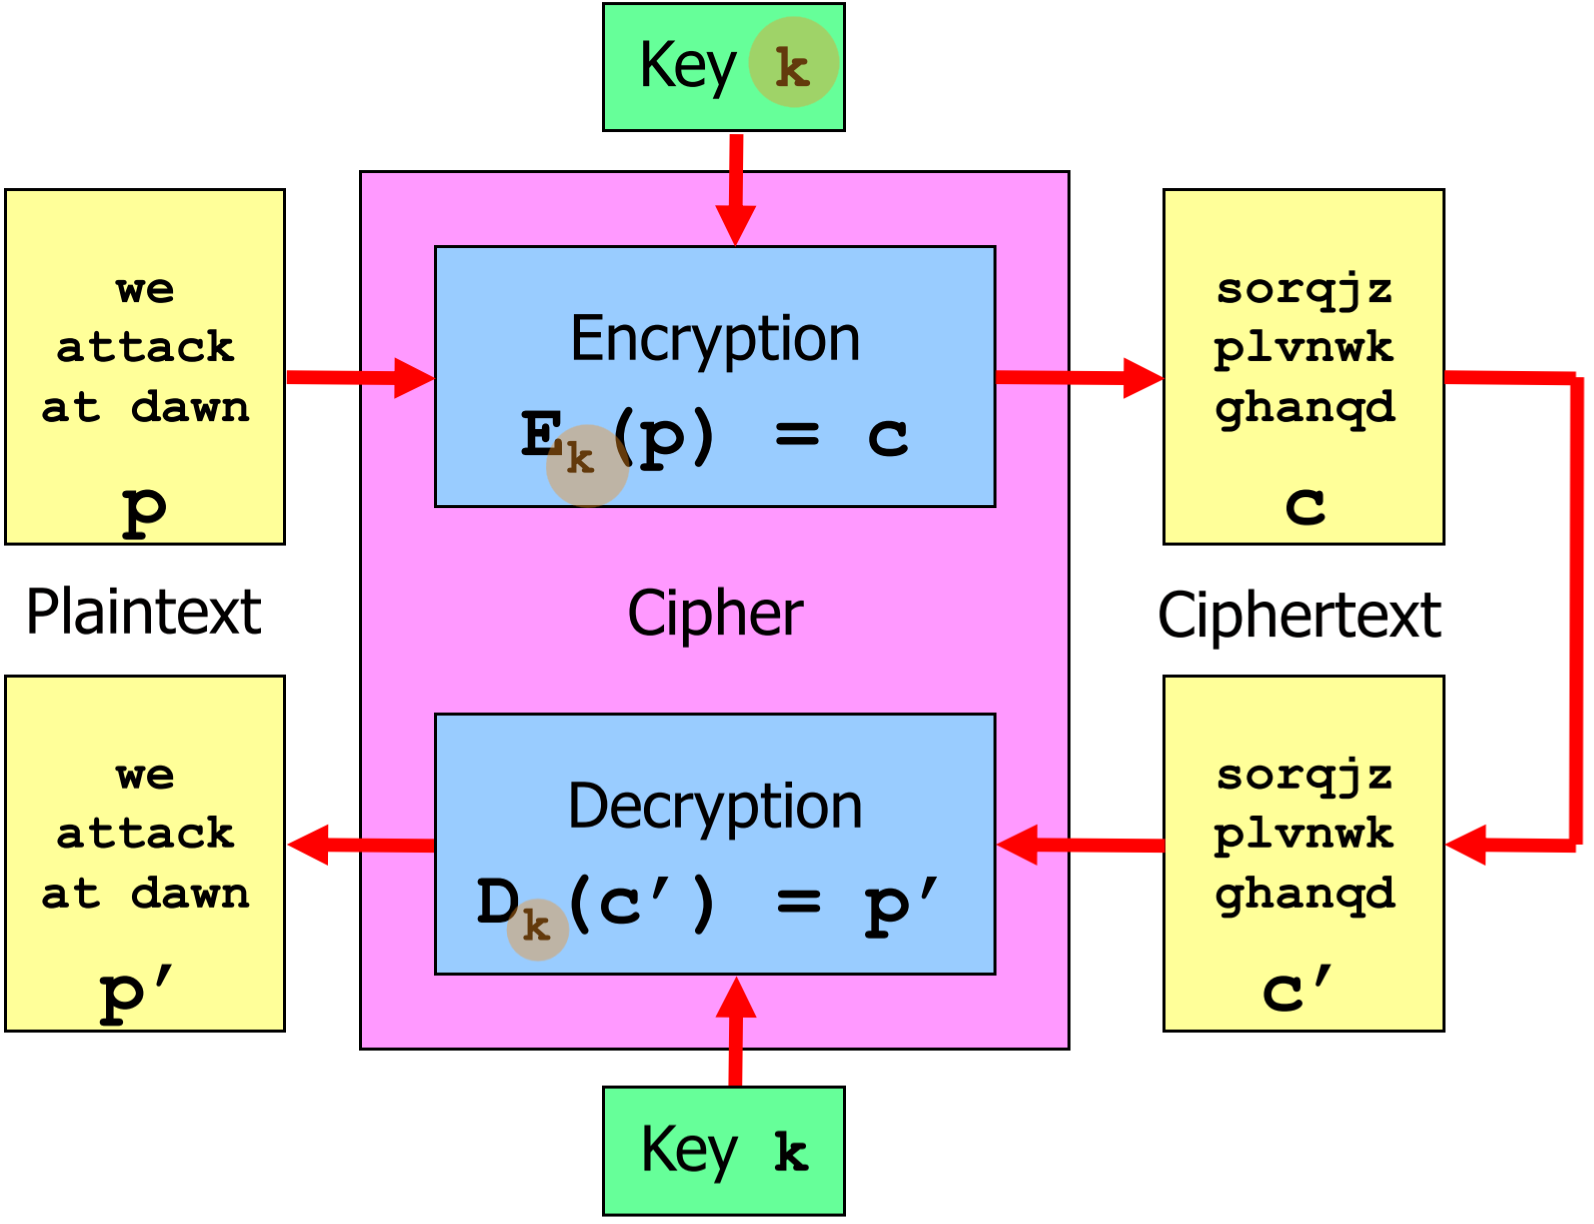
\includegraphics[width=150px]{img/BasicTerminologySecKeyCrypto.png}
%        \captionof{figure}{Basic Terminology basierend auf Secret Key Cryptography}
%        \label{fig:Basic Terminology}
%    \end{Figure}

\tableofcontents

\newpage

\chapter{Einführung}

\section{Weshalb Recht?}
Jede Gesellschaft braucht Regeln, deshalb gibt es Recht.
\begin{itemize}
   \item Social Framework
   \item Konfliktmanagement $\rightarrow$ nicht jeder Konflikt endet in einem Streit
   \item erhält Werte 
   \item sichert Freiheit  
   \item schafft Rahmen zur sozialen Integration $\rightarrow$ für neue Personen welche in ein Land kommen
   \item schafft gleiche Rahmenbedingungen für alle Marktbeteiligten $\rightarrow$ Gerade sehr wichtig für die Informatik. Wenn beispielsweise die Swisscom immer mehr Brandbreite erhält wie Salt, so hat Salt tendenziell schlechteres Netz / Empfang.
   \item legitimiert staatliche Organe wie Behörden oder Gerichte 
   \item steuert und gestaltet die gesellschaftlichen Akteure
   \item Machtkontrolle
   \item Zwingt jeden, seinen Willen präzise auszudrücken
\end{itemize}

\subsection{Bedeutung von Recht in einem technischen Umfeld}
\begin{itemize}
   \item Recht als Rahmen des Zulässigen (\textbf{= Maximum}) oder des rechtlich Verlangten (\textbf{=Minimum}) innerhalb eines (sozialen) Systems
   \item Klärung der Verpflichtung und Verantwortlichkeiten/Haftung
   \item Industrie-Standards / Best-Practices ergänzen das Recht $\rightarrow$ beispielsweise ISO-Standards
   \item ABER: Standards/Best-Practices klären oft nicht ausreichend alle rechtlichen Fragen (bspw. Cloud-Verträge)
\end{itemize}

\subsection{Recht als Risk-Management}
\begin{itemize}
   \item Um Risiken zu handlen ist es sinnvoll, sowohl \textit{technische} (by Design), \textit{organisatorische} (bspw. 4-Augen Prinzip) und \textit{rechtliche} Massnahmen (bspw. vertragliche Absicherung) zu treffen
   \item Holen Sie sich rechtliche Unterstützung \textit{so früh wie möglich} $\rightarrow$ andernfalls können Projekte in letzter Minute abgeschossen werden
   \item Das Management ist persönlich verantwortlich, die Einhaltung von rechtlichen Vorschriften zu organisieren und zu kontrollieren (Compliance)
\end{itemize}
Die Personen, welche an der Front arbeitet oder im direkten Kundenkontakt stehen, sind als erstes diesen Risiken ausgesetzt.\\
\textbf{Grundsatz:} Alles was zu Beginn nicht ausdiskutiert wird, kommt zu einem späteren Zeitpunkt nochmals auf's Tapet, zu diesem Zeitpunkt, dann jedoch unter anderen Rahmenbedienungen.

\subsection{zentrale (Obligationen-) rechtliche Frage}
Ist eine einfache Vorgehensweise, wie ich Situationen einmal einschätzen kann.\\
Bei Verträgen muss man diese Fragen sehr schnell, in einer möglichst genauen Formulierung formulieren 
\begin{enumerate}
   \item \textbf{WER} will
   \item von \textbf{WEM}
   \item \textbf{WAS}
   \item \textbf{WORAUS}
\end{enumerate}
\textbf{merke:} Wenn eine Behauptung juristisch begründet werden kann, erhöht dies die Macht und es muss nicht mehr diskutiert werden.

\subsection{Sitte, Moral, Recht}
Sitte $\rightarrow$ eine gemeinsame Regel, welche aber nicht zwingend durchgesetzt werden können\\
Moral $\rightarrow$ \\
Recht $\rightarrow$ gesetzlich verankert
\begin{itemize}
   \item Sich zum Teil überschneidende, sozial gewünschte Verhaltensweise
   \item Recht muss sich veränderten Verhaltensweise immer wieder anpassen
   \item Rechtliche Verbindlichkeit ist in einer vielfältigen, offenen Gemeinschaft für alle einzufordern (grösster gemeinsamer Nenner)
\end{itemize}
\begin{Figure}
   \centering
    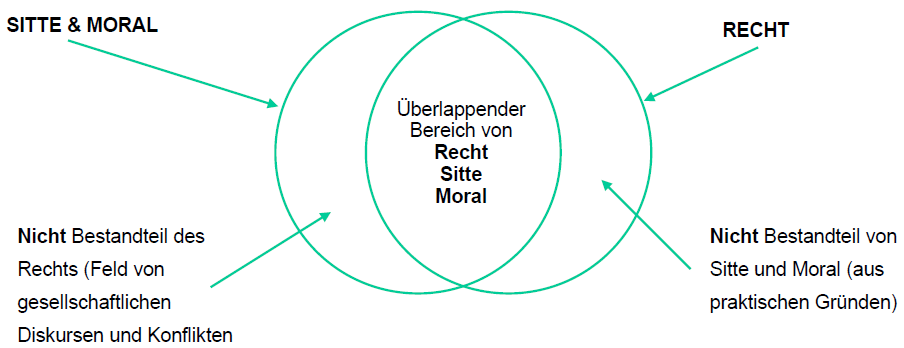
\includegraphics[width=150px]{img/SitteMoralRecht.png}
        \captionof{figure}{Zusammenspiel zwischen Sitte, Moral und Recht}
        \label{fig:Sitte Moral Recht}
\end{Figure}

\section{Weitere Ausführungen}

\subsection{juristische Argumentation}
$\Rightarrow$ \textbf{Behauptung} wird durch \textbf{Grundlage} (Gesetztesartikel) und \textbf{notwendigen Beweis} gestützt \\
oder \\
$\Rightarrow$ \textbf{Gestützt auf Grundlage} (Gesetztesartikel) und notwendigem \textbf{Beweis} ergibt sich die Schlussfolgerung

\subsection{Gewaltentrennung}
Auf eidgenössischer, kantonaler und kommunaler Ebene gibt es jeweils drei unabhängige Instituationen:
\begin{itemize}
   \item Legislative (bspw. Ständerat)
   \item Exekutive (bspw. Polizei)
   \item Judikative (bspw. Gerichte)
\end{itemize}
$\rightarrow$ Jede dieser Autoritäten kontrolliert und balanciert die Macht der anderen beiden.

\subsection{Rechtsordnung unter verschiedenen Blickwinkeln}
\begin{itemize}
   \item Rang $\rightarrow$ Verfassung, Gesetz, Verordnung
   \item erlassendem Gemeinwesen $\rightarrow$ Bundesrecht, kantonales- und Gemeinderecht
   \item Rechtsquelle $\rightarrow$ geschriebenes Recht, Gewohnheitsrecht, Gerichtspraxis, ZGB 1
   \item Beteiligten Personen $\rightarrow$ Privatrecht, öffentliches Recht
\end{itemize}

\subsection{Bund, Kantone, Gemeinden}
\begin{itemize}
   \item \textit{Das Schweizervolk und die Kantone, bilden die Schweizerische Eidgenossenschaft} (Art. 1 BV) und nicht umgekehrt
   \item \textit{Das Kantonsgebiet gliedert sich in Gemeinden} (z.B. §6 Kantonsverfassung LU)
   \item Bund darf nur Gesetze erlassen und in einem Rechtsbereich handeln, wenn es dazu eine verfassungsmässige Legitimation gibt
   \item Kantone stehen in der Gesetzgebungsmacht über dem Bund! Kanton über den Gemeinden
\end{itemize}

\begin{Figure}
   \centering
    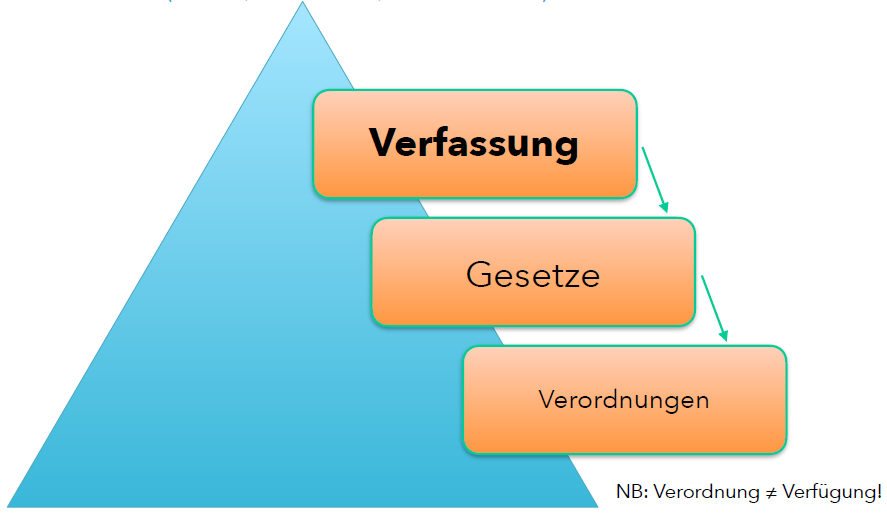
\includegraphics[width=300px]{img/RechtsHierarchie.png}
        \captionof{figure}{Hierarchie der Rechte}
        \label{fig:Rechtshierarchie }
\end{Figure}

\subsection{Privat- / öffentliches Recht}
Es unterscheidet völlig unterschiedliche Gerichtsbarkeit (Zivil- / Verwaltungsgericht) mit unterschiedlichen Prozessabläufen und Prozessrechten.\\
Privatrecht wird vom Grundatz der \textbf{Koalitions- und Vertragsfreiheit} beherrscht, öffentliches Recht dagegen vom \textbf{Legalitätsprinzip} (Gewaltenkontrolle)
\textbf{Privatrecht}\\
\begin{itemize}
   \item Bürger gegen Bürger
   \item OR / ZGB
   \item GeBüV
   \item DSG
   \item URG, UWG, u.a.m
   \item $\rightarrow$ Erbrecht, gibt zwar Vorgaben kann jedoch verhandelt werden
\end{itemize}

\textbf{öffentliches Recht}
\begin{itemize}
   \item Staat gegen Bürger
   \item StGB
   \item FMG
   \item BÜPF/VÜPF
   \item EIDI-V u.a.m
   \item $\rightarrow$ Drogen verkaufen ist illegal und wir geahndet. Kann nicht verhandelt werden.
\end{itemize}

\subsection{Rechtsbegriffe}
\begin{itemize}
   \item Zwingendes, vereinbartes und dispositives Recht
   \subitem zwingendes Recht: Vorschriften die nicht durch einen Vertrag wegbedungen werden können. I.d.R. Vorschriften die öffentliche oder Dritten Interesse dienen. $\Rightarrow$ Muss immer erfüllt werden, bspw. Schriftlichkeit bei Mietkündigung
   \subitem dispositives Recht: Können durch Verträge wegbedungen werden $\Rightarrow$ greift, wenn nichts anderes vereinbart, bspw. Kündigungsfrist bei Arbeitsvertrag 
   \item Vermutung des guten Glaubens (ZGB 2)
   \item Handeln nach Treu und Glauben
   \item Richterliches Ermessen (ZGB 4)
   \item Beweislast (ZGB 8)
   \subitem Kläger A behauptet etwas, Beklagter B antwortet. Das Gericht sagt: A muss x,y,z beweisen und B muss r,t beweisen. 
\end{itemize}

\subsection{ausländisches Recht}
Nebst dem Völkerrecht und internationalen Verträgen, ist das \textbf{IPRG} (Gesetz über das internationale Privatrecht) die Hauptschnittstelle zwischen CH und ausländischem Recht.
Das IPRG regelt, wann welches Recht (CH oder Ausland) anwendbar ist und welche Richter zuständis sein sollen.

\section{Essentials / das wichtigste in Kürze}

\subsection{Instanzenzug}
\begin{itemize}
   \item Es reicht nicht zu wissen, welche Rechte man hat, man muss auch wissen, wie man diese \textbf{durchsetzen} kann
   \item Zivil-, Verwaltungs-, Strafgericht haben unterschiedliche Verfahren
   \item Grundsätzlich aber in allen Rechtsbereichen drei Instanzen: Bezirksgericht - Kantonsgericht - Bundesgericht
\end{itemize}

\subsection{Essentials Zivilprozess}
\begin{itemize}
   \item Vermittlungsverfahren mit Friedensrichter
   \item Vor dem örtlich / sachlich zuständigen Gericht
   \item in Zivilverfahren muss regelmässig ein Gerichtskostensvorschuss, der vom Streitwert abhängt, bezahlt werden
   \item In Zivilverfahren muss der Kläger den behaupteten Anspruch beweisen, das Gericht sucht keine Beweise
   \item Wer den Zivilprozess verliert, muss die Gerichtskosten sowie Parteikosten der anderen Seite übernehmen
   \item Wer einen Forderungsprozess gewinnt, hat das Geld noch nicht (je nachdem kann das Unternehmen zum Beispiel gar nicht bezahlen, wenn es Konkurs geht)
\end{itemize}

\subsection{Essentials Strafverfahren}
\begin{itemize}
   \item Verfahren sind in StGB und StPO geregelt. Polizei unterliegt überwiegend kantonaler Hoheit und ist dort geregelt
   \item Örtliche Zuständigkeit ergibt sich aus dem Tat- oder Erfolgsort
   \item Für Antragsdelikte gilt eine Frist von 3 Monaten
   \item Staatsanwalt (StA) leitet Untersuchung, muss belastend und entlastende Aspekte sammeln
   \item Als Opfer hat man nur begrenzte Einsicht in Untersuchungsmassnahmen. Ausser man bringt isch als Privatstrafkläger ein
   \item StA stellt entweder Verfahren ein, straft (max 6 Monaten Freiheitsstrafen und oder 180 Tagessätze) oder überweist den Fall zur Beurteilung an das Strafgericht
\end{itemize}

\subsection{Essentials Verwaltungsverfahren}
\begin{itemize}
   \item Verfügungen müssen durch die richtige Behörde im richtigen Verfahren und unter Angabe der Rechtsmittels dagegen erlassen werden. Sonst ist die Verfügung nichtig.
   \item Grundsätzlich immer wiedererwägung/Einsprache gegen die Verfügung möglich, wenn neue Tatsachen auftauchen
   \item Gegen Verfügungen kann i.d.R. Beschwerde inner 10/20/30 Tagen geführt werden
   \item Je nach Gesetzesgrundlage ist kantonales Obergericht oder Bundesgericht die höchste Instanz.
\end{itemize}




\chapter{IT-Verträge}
Grundsätzlich gilt bei Verträgen, alles was am Anfang nicht verhandelt wird, wird zu einem späteren zeitpunkt wieder verhandelt werden - dann aber bei anderen Rahmenbedienungen

\section{Allgemeines zu Verträgen}
\begin{itemize}
   \item Es geht um die Beweisbarkeit von Abschluss und Inhalt von Rechtsgeschäften mittels Zeugen, Schriftlichkeit, Siegel, handschriftliche oder elektronische Signaturen
   \item Voraussehbare, einheitliche Regeln (Standards) zur Lückenfüllung und Durchsetzung der Verträge erleichtern den Handelsverkehr
   \item Schutz einer Parter vor Übervorteilung
   \item Schutz des fairen Wettbewerbes
   \item Bei allem gilt \textbf{Grundsatz der Vertragsfreiheit (Form und Inhalt)}
   \subitem Es gibt jedoch ein paar Einschränkungen (bspw. übermässige Bindung) 
\end{itemize}

\subsection{Internationale Zusammenarbeit}
Rechtsgeschäfte zwischen weltweit verteilten, sich nicht kennenden Parteien schaffen neue (praktische und rechtliche) Probleme:
\begin{itemize}
   \item Dauerverträge für Online-Services $\rightarrow$ Was passiert, wenn man keinen Zugang mehr hat?
   \item Agile Projektentwicklung braucht klare Rahmen
   \item Daher sind in der Praxis nicht nur Verträge im klassischen Sinne relevant
\end{itemize}

\subsection{Übliche Fragen bei Verträgen}
\begin{itemize}
   \item Was war Inhalt des Vertrages?
   \item Einigkeit über alle relevanten Vertragspunkten?
   \item Wann ist der Vertrag korrekt erfüllt?
   \item Zahlungsmodalität?
   \item War die vertragschliessende Partei berechtigt, den Vertrag abzuschliessen? (Vollmacht der Firma etc)
   \item Beweis- und Aufbewahrungspflicht?
   \item Wer sass tatsächlich vor dem Computer?
   \item Wann wurde der Vertrag geschlossen?
   \item Wie sieht das im internationalen Verkehr aus?
\end{itemize}
$\rightarrow$ Oftmals beginnt man mit einem kurzen Vertrag der verpflichtend ist und verhandelt zu einem späteren Zeitpunkt die Details aus. 

\subsection{Pacta Sunt servanda vs. Flexibilität}
\textbf{Grundsatz:} Verträge mit dem einmal vereinbarten Inhalt sind bindend\\
\textit{Ausnahmen:}
\begin{itemize}
   \item Parteien ändern gemeinsam Inhalt (Konsens)
   \item Erfüllung ist (objektiv) unzumutbar geworden
   \item Bei vertraglichen Lücken: hypothetischer Parteiwille wird angenommen
\end{itemize}
\textit{frühzeitiges kreatives Weiterdenken}
\begin{itemize}
   \item Wo und wie könnten sich die Vertragsgrundlagen ändern?
   \item Wie kann der Vertrag zweckmässig angepasst werden?
   \item Wahlmöglichkeiten der benachteiligten Partei
   \item Objektivierte Weiterentwicklung wie Index, Berechnungsformeln etc.
   \item Verpflichtung zu Vertragsverahdnlung (mit Deadlock bei Nichteinigung)
\end{itemize}

\subsection{Tailor-Made-Verträge vs. Musterverträge}
\textbf{Grundsatz:} Nie ein Muster verwenden ohne es entsprechend zu reflektieren und auf den aktuellen Kontext zu beziehen
\begin{itemize}
   \item Richtige Rechtsordnung?
   \item Vergleichbarkeit der Sachverhalte?
   \item Enthält das Muster auch relevanten Regelungen?
   \item Sind Änderungen der Rechtslage berücksichtigt?
   \item Sind die richtigen Namen enthalten :-)
\end{itemize}
$\rightarrow$ Immer sich hinterfragen ob ein Standardvertrag nicht ausreicht oder ob es tatsächlich keinen Tailor-Made-Vertrag braucht.

\subsection{Vertragsgestaltung}
\begin{itemize}
   \item KISS - \textbf{K}eep \textbf{I}t \textbf{S}imple and \textbf{S}tupid $\rightarrow$ but not too much!
   \item einfach, klar und verständliche (bspw. Begriffe definieren)
   \item Unterscheidung zwischen Motiv (Einleitung, zu welchem Zweck) und Verpflichtung
   \item Prozessbezogenes Denken
   \subitem Wie läuft die gegenseitige Leistungserfüllung ab?
   \subitem Welche Rechte haben die Parteien, wenn eine Leistung nicht erfüllt wird? 
   \item An Beginn \textbf{und} Ende der Zusammenarbeit denken (Exit-Klausel, Mitwirkungspflichten bei Hosting oder SaaS etc.)
   \item pacta sunt servanda vs. Flexibilität und Abänderbarkeit des Vertragsverhältnisses
   \item Tailor-made vs. Mustervertrag
   \item In der IT oftmals ein Rahmenvertrag, mit einem Side-Letter 
   \subitem regelt Rahmenbedienungen 
\end{itemize}

\subsubsection{Checkliste Vertragsinhalt}
\begin{itemize}
   \item Spezifikation Vertragsleistung
   \subitem Beim Verzug ist Voraussetzung, dass man die andere Partei vorgängig informiert, dass man zu diesem Zeitpunkt mit der Leistung rechnetve 
   \item Preis, Zahlungsbedingungen
   \item Erfüllgszeit- und ort
   \item Abnahmeverfahren
   \item Vorgehen bei Mängel, Nachbesserung
   \item Haftung für Mängel
   \item Konventionalstrafe
   \item Geheimhaltung, Datenschutz
   \item Gerichtsstand, anwendbares Recht
\end{itemize}

\section{Offerte und Vertragsabschluss}
\textbf{Art. 1 OR:} \textit{Vertrag kommt durch gegenseitige, übereinstimmende Willensäusserung zustande. Diese kann ausdrücklich oder stillschweigend erfolgen}\\
\textbf{Offerte:} verbindlicher Antrag, den Vertrag unter bestimmten Bedingungen (Preis, Menge etc.) abschliessen zu wollen\\
\textbf{Akzept:} Annahme der Offerte\\
$\Rightarrow$ Verbindliche Offerte oder bloss Einladung zur Offertstellung (Art. 7 OR)\\
Bspw.: Bestellvorgang beim Online-Handel ist beim Klicken auf den Bestell-Knopf die Offerte. Vorher handelt es sich um eine Einladung zur Offertstellung.\\
\textbf{Einladung zur Offertstellung:} Der Vertrag kommt erst Zustande, wenn der Anbieter eine Bestätigung gibt (Anbieter kann damit zuerst noch bspw. Bonität oder Lagerbestand prüfen). Somit ist dies nur ein bekunden von Interesse des Kundens.

\subsection{Vertragsformen}
\textbf{Art. 11 OR:} Verträge sind grundsätzlich nicht an eine Form gebunden, ausser dies wird vom Gesetzt verlangt\\
\textit{Stufen}
\begin{enumerate}
   \item Formlos $\rightarrow$ Einkauf bei Migros
   \item Einfache Schriftlichkeit $\rightarrow$ Testament
   \item Qualifizierte Schriftlichkeit $\rightarrow$ Lehrvertrag
   \item Öffentliche Beurkundung $\rightarrow$ Ehevertrag, Erbvertrag, Hauskauf
   \item Eintrag in ein öffentliches Register $\rightarrow$ AG Gründung
   \item Öffentliche Beurkundung und Eintrag in ein öffentliches Register
\end{enumerate}

\subsection{Einteilung Verträge}
\textbf{Nominatverträge:} gesetzlich geregelte Vertragsformen - zwingend oder dispositives $\rightarrow$ klare Regelung\\
\begin{itemize}
   \item Kaufvertrag $\rightarrow$ Standardsoftware, Infrastruktur
   \item Auftrag $\rightarrow$ Consulting, Installation, SLA etc.
   \item Werkvertrag $\rightarrow$ kundenspezifische Software, Infrastruktur
   \item Miete $\rightarrow$ Hardware
   \item Zusammengesetzt Verträge $\rightarrow$ Hosting, Projektumsetzung, Entwicklung
   \item Arbeitsverträge
\end{itemize}

\textbf{Innominatverträge:} gesetzlich \textbf{NICHT} geregelte Vertragsformen - Vertragsfreiheit $\rightarrow$ bei Unklarheiten entscheidet das Gericht in der Regel analog zum dominierenden Nominatvertrag
\begin{itemize}
   \item Leasing
   \item Lizenzvertrag
   \item Factoring-Vertrag $\rightarrow$ Faktura: Rechnungsverträge
   \item Escrow-Agreement $\rightarrow$ Source-Code wird deponiert, Software-Unternehmen muss den Source-Code bei einem Escrow-Agent (Treuhänder) hinterlegen, um bei bspw. Konkurs auf den Source-Code zugreifen zu können
   \item Software-Entwicklungsvertrag $\rightarrow$ typische Regelung, das Risiko wird durch beide Parteien geteilt
   \item Service level Agreement (SLA)
\end{itemize}

\section{Typische Fälle wo es schwierig wird}
\begin{itemize}
   \item (angeblich) keine oder zu späte Lieferung
   \item Mangelhaftes Produkt/Garantieleistung (man kann oft nicht sehen was die Spezalisten gemacht haben und ob es gut ist.)
   \item Fehlende Zahlung (bspw. Betreiben ist oft schwierig, da man sonst den Kunden verliert)
   \item Mehrere ander Leistungserfüllung Beteiligte
   \item Unklares Abnahmeverfahren
   \item Übermässige Bindung
   \item Andere Mängel (Nichtigkeit, Unmöglichkeit, Übervorteilung) $\rightarrow$ Immer Beweismittel produzieren
\end{itemize}

\subsection{Anfechtbar vs. nichtig}
\begin{itemize}
   \item \textbf{Anfechtbarer Vertrag:} Gültiger Vertrag und bleibt gültig, solange sich die benachteiligte Vertragpartei nicht innerhalb eines Jahres wehrt und sich auf Willensmangel beruft (absichtliche Täuschung). Der angefochtene Vertrag wird dann aufgehoben oder abgeändert.
   \item \textbf{nichtiger Vertrag:} Ein nichtiger Vertrag gilt als nicht abgeschlossen. Die Staatlichen Zwangsmittel (bspw. Prozess) können zur Durchsetzung eines Anspruches nicht eingesetzt werden.
\end{itemize}

\section{Verzug}
Verzug heisst, jemand der für eine Leistung verpflichtet ist, ist spät dran. Es ist nicht immer lohnenswert direkt mit Grossszenarien zu drohen.\\
\textbf{Art. 91 und 102 OR:} Gläubiger- und Schuldnerverzug\\
\textbf{Verzung und Mahnung:} normalerweise erst mit ausdrücklichem Hinweis wird ein Verzug ausgelöst, dass die geschuldete Leistung nun fällig ist\\
\textbf{Art. 103 ff. OR:} Verzugsfolgen allgemein\\
\textit{Merke:} Mahnläufe sind nicht Pflicht, es kann beim Verzug direkt betrieben werden.


\subsection{Schlecht- oder Nichterfüllung}
Grundsätzlich kommt dem Anbieter als Spezialist eine besondere Aufklärungspflicht und Haftung zu $\rightarrow$ 
\textbf{Wichtig} Produktivnutzung der Software impliziert regelmässig, dass das System tauglich ist und über keine grösseren Mängel verfügt.
\begin{itemize}
   \item Nichterfüllung: Ich kann nicht arbeiten
   \item Schlechte Erfüllung: Ich kann arbeiten aber nicht sehr produktiv und es fehlt viel
   \item Kleinere Mängel und Anpassungen: bspw. Schreibfehler
   \item $\rightarrow$ Wenn die Software produktiv bedient wird, gilt sie als abgenommen auch wenn es noch kleinere Mängel hat
\end{itemize}
\textbf{Art. 197 und 367 OR:} Mängelrügen \\
Nichterfüllung $\neq$ Schlechterfüllung\\


\section{Verträge im Informatikkontext}

\subsection{Software-Entwicklung}
\textbf{Klassisch}: Pflichtenheft, Meilensteine und Abnahme = Werkvertrag und Lizenz- und Kaufvertrag\\
\textbf{agile}: \\
Werkvertrag? $\rightarrow$ Resultat zählt\\
Auftrag? $\rightarrow$ Dienstleistung zählt\\
Einfache Gesellschaft? $\rightarrow$ Zusammenarbeit für das Erreichen eines bestimmten Zwecks

\begin{Figure}
   \centering
    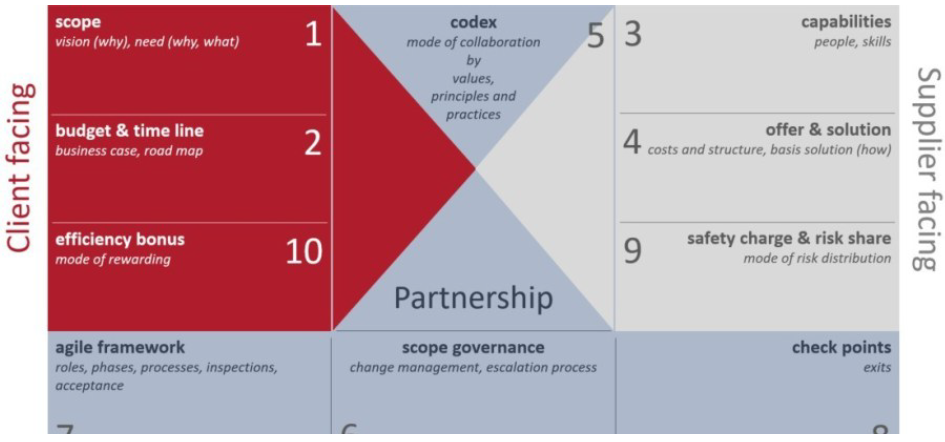
\includegraphics[width=150px]{img/agileVertragsgestaltung.png}
        \captionof{figure}{Vorgehen Vertragsgestaltung für agile Projekte}
        \label{fig:agile Vertragsgestaltung}
\end{Figure}

\subsection{Einzelne Verträge}

\subsubsection{Werkvertrag}
Unternehmer verpflichtet sich zur Erstellung eines Werkes gegen Entgelt.
\begin{itemize}
   \item Bestimmung des Preises $\rightarrow$ Fixpreis, nach Aufwand, Kostendach
   \subitem Es sollte geregelt werden, was beim Überschreiten des vereinbarten Preises passiert 
   \item Gewährleistungspflichten $\rightarrow$ Abnahmeverfahren des Werkes in vereinbarter Qualität am Schluss, Garantie i.d.R. analog Kaufvertrag
   \item Rücktritt und Schadenersatz $\rightarrow$ Hat der Besteller Rücktrittsrecht und was kostet ihn das?
\end{itemize}

\subsubsection{Auftragsverhältnis}
Tätig werden im Interesse des Auftraggebers. Es ist kein Resultat geschuldet
\begin{itemize}
   \item kann jederzeit beendet werden (Art. 404 OR) $\rightarrow$ gilt jedoch nicht bei atypischen Verträgen mit Kündigungsfrist wie bspw. Support-Vertrag
   \item Rechenschaftspflichts des Auftragnehmers $\rightarrow$ Auftragnehmer zeigt dem Auftraggeber was er unternommen hat
   \item Haftung für Handeln im Interesse des Auftraggebers. Aber keine Haftung für den Eintritt eines bestimmtes Erfolges
\end{itemize}

\subsubsection{Einzelarbeitsvertrag}
Inhalt und Abgrenzung zu Auftrag, Werkvertrag, Agenturvertrag, einfache Gesellschaft
Arbeitnehmer, Selbstständig oder Scheinselbständig $\rightarrow$ Indizien für Anstellungsverhältnis:
\begin{itemize}
   \item regelmässige und dauerende Tätigkeit für denselben Auftraggeber
   \item Ein- bzw. Unterordnung in einer Projektorganisation des Auftraggebers
   \item kein Tragen unternehmischer Risiken
   \item weder mit Kundenakquisition noch mit Projektmanagement befasst
   \item Dem Kunden gegenüber für Projektausführung und allfällige Mängel nicht verantwortlich
   \item Inkasso nicht selbständig durchführen
\end{itemize}
Der Arbeitnehmer verpflichtet sich seine Kapazität dem Arbeitgeber zur Verfügung zu stellen.

\textbf{Typische Fragen des Arbeitsrechtes}
\begin{itemize}
   \item Zustandekommen, Kettenverträge, (un)befristet 
   \item Lohn, Leistungslohn, Bonus
   \item Überstunden, Kompensation
   \item Probezeit, Kündigung
   \item Lohnfortzahlung, Krankheit, Militär
   \item Nachvertragliche Konkurrenzverbote
   \item Haftpflicht
   \item Arbeitszeugnis
   \item ArG (Anwendbarkeit, Gesundheitsschutz, Arbeits- und Ruhezeiten, Familienpflichten)
\end{itemize}

\textbf{MERKE!}\\
Eine Kündigung ist eine einseitige, empfangsbedürftige Erklärung

\subsubsection{Personalverleih (Bodyleasing)}
\begin{itemize}
   \item AVG (BG über die Arbeitsvermittlung und den Personalverleih)
   \item Bewilligungspflichtiges Gewerbe mit Pflicht zur Hinterlegung einer Kaution
   \item Regelmässige Fragen zu Weisungsrecht, Kündigung und Konkurrenzverbot
\end{itemize}

\subsubsection{Zusammenarbeitsverträge}
\begin{itemize}
   \item Händlervertrag (Vertriebsvertrag)
   \item Agenturvertrag
   \item \textbf{Achtung!} Einfache Gesellschaft (Haftung)
\end{itemize}

\section{Arbeitsverträge}
Arbeitsverträge können auch stillschweigend erfolgen. Es muss nicht schriftlich sein bspw. Beförderung.

\subsection{Überstunden vs. Überzeit}
Überstunden $\neq$ Überzeit! 
\begin{itemize}
   \item Bis 50h (mehr als vereinbart) = Überstunden
   \item Über 50h (mehr als vereinbart) = Überzeit
   \item Dabei ist die Kompensation \textbf{immer} freie Zeit in mind. gleicher Länge
   \subitem Ausnahme 1: Zu wenig Zeit übrig für freie Zeit bei einer Kündigung
   \subitem Ausnahme 2: Bei Teilzeitarbeitenden
   \item Ein Verfallen der Überstunden ist in der Schweiz nicht zulässig - unabhängig was im Vertrag steht
   \subitem Ausnahme 1: Jahresarbeitszeit - Verantwortung geht an den Arbeitnehmer. Aber wenn die Freiheit nicht geboten wurde (wenn keine Möglichkeit auf Kompensation bestand, muss es ausbezahlt werden)
   \item Die Verjährungsfrist für finanzielle Arbeitsrechtliche Forderungen ist 5 Jahre   
\end{itemize}

\subsection{Probezeit, Kündigung}
Eine Kündigung ist eine einseitige, empfangsbedürftige Erklärung.\\
Bei befristigten Verträgen, gibt es keine Kündigung, da der Vertrag einfach ausläuft\\

\begin{itemize}
   \item Einsitige Erklärung: Der Arbeitgeber muss die Kündigung nicht akzeptieren.
   \item empfangsbedürftige Erklärung: Sie muss empfangen worden sein. Es ist nicht notwendig, dass der Vorgesetzte das mitbekommt. 
   \subitem Es kann auf dem falschen Tisch landen, so lange es empfangen wurde
   \item Kündigungen können nicht zurückgenommen werden
   \item Während Probezeit darf man in die Ferien
   \item Wenn man nach der Lehre im gleichen Unternehmen bleibt, so darf keine Probezeit vereinbart werden.
   \item Beim Rollenwechseln in der gleichen Unternehmen, kann eine Probezeit vereinbart werden
   \item Während der Probezeit gibt es keinen Kündigungsschutz
   \item Kündigungen gehen nur bei offenen (nicht befristet) Verträgen (ausser fristloser Kündigungen)
\end{itemize}

\subsection{Lohnfortzahlung bei Krankheit, Militär und Unfall}
\begin{itemize}
   \item OR: Ab dem ersten Tag 100\% während einer bestimmten Dauer, abhängig von der Anzahl Jahre im Unternehmen
   \item Meisten Unternehmen haben eine Versicherungslösung, welche die Lohnfortzahlung (bis es zum IV-Fall wird $\rightarrow$ 720 Tage) gewährleistet 
\end{itemize}

\subsection{Konkurrenzverbot}
\begin{itemize}
   \item Nachvertragliches Konkurrenzverbot $\rightarrow$ Wenn sie kündigen, dürfen sie nicht zur Konkurrenz
   \item Gilt nur wenn der Arbeitnehmer kündigt, ansonsten verfällt es
   \item Muss drei Dinge beschreiben:
   \subitem 1) Räumlich: In welcher Lage darf nicht gearbeitet werden (die Berufsausübung muss noch möglich sein)
   \subitem 2) Sachlich: in welcher Rolle (enge Umschreibung der Funktion)
   \subitem 3) zeitlich: in welchem Zeitraum (max. 3 Jahren) 
   \item Je spezialisierter man ist, desto weniger kann einem das Konkurrenzverbot gefährlich werden.
\end{itemize}

\subsection{Haftpflicht}
\begin{itemize}
   \item Normalerweise haftet der ARbeitgeber
   \item In Spezialfällen aber der Arbeitnehmer (müssen alle 3 zutreffen)
   \subitem 1) Wenn der Arbeitgeber den Arbeitnehmer beauftragt hat, weil er Fachmann ist und das können muss
   \subitem 2) Der Arbeitgeber muss instruiert haben und ihn auf Risikien hingewiesen haben
   \subitem 3) Der ARbeitgeber muss den Arbeitnehmer überwachen. 
\end{itemize}

\subsection{Arbeitszeugnis}
\begin{itemize}
   \item Es kann jederzeit ein Arbeitszeugnis verlangt werden
   \item Das Schlusszeugnis muss sich auf das gesamte Arbeitsverhältnis beziehen
   \item Müssen Wohlwollend formuliert sein, vollständig und wahr
\end{itemize}



\chapter{IT-Verträge konkret: Lizenzvertrag und Urheberrecht}
Es geht dabei nicht nur um Softwarelizenzverträge. Es geht um nicht-materielle Vereinbarungen. Nicht nur Nutzung einer Software, sondern acuh NUtzung eines Markenrechtes
\section{Beschaffungsverträge}
$\rightarrow$ Ziel: Eigentumswechsel oder dauerhaftes Nutzungsrecht
\begin{itemize}
   \item Kauf 
   \item Werkvertrag
   \item Dienstleistungsvertrag ('Service')
   \item \textbf{Lizenzvertrag (Nutzungsrecht / 'Miete')}
   \item GU-Vertrag
   \item Outsourcing
\end{itemize}

\section{Lizenzverträge}
\begin{itemize}
   \item Sind gesetzlich nicht geregelt
   \item Lückenfüllung falls notwendig i.d.R. aus Mietvertragsrecht, Auftragsrecht und Werksvertragsrecht
   \item Anwendungsbereich
   \subitem Software, Patente, Markenrechte, Urheberrecht, Nutzung von Plattformen, Vertriebsverträge, Kooperationsverträge etc. 
\end{itemize}

\textbf{Typische Lizenzbestimmung:} \textit{Der Lizenzgeber gewährt dem Lizenznehmer ein zeitlich
unbegrenztes, nicht übertragbares, nicht ausschliessliches
Recht, den Lizenzgegenstand in der zum Zeitpunkt des
Vertragsschlusses aktuellen Version zu nutzen.“}\\

\subsection{Haftung}
Wenn ein Schaden entsteht, muss dieser ausgeglichen werden. Normalerweise steht in einem Vertrag:
\textit{i.d.R. wird jegliche Haftung für Schäden im Rahmen des gesetzlich zulässigen (OR Art. 100) ausgeschlossen! Verursacher haftet in solchen Fällen nur, wenn der Schaden grob fahrlässig oder vorsätzlich (mit Wissen und Wollen) verursacht wurde}\\

Wenn ein Jurist von Schaden/Schadenersatz spricht, so ist es immer eine Vermögensdifferenz. Bspw. Wert des Fahrzeuges vor der Verformung und nach der Verfomung $\rightarrow$ Schaden.
\begin{itemize}
   \item Allfällige ungültige Bestimmungen sollen im Sinn der Fortführung des Vertrages ersetzt werden
   \item Ausschluss allgemeiner Geschäftsbedingungen (AGB)
   \item Schlichtungs-/Mediationsformel
   \item Anwendbares Recht und Gerichtsstand
\end{itemize}



\subsection{Open-Source}
Man unterscheidet zwischen
\begin{itemize}
   \item strengen Copyleft (GNU, GPL, SIK)
   \subitem Weiterentwicklung muss ebenfalls Open-Source sein
   \item Non-Copyleft (Apache, MIT, BSD) 
   \subitem Entwicklung darf frei verwendet und geändert werden
   \subitem Darf verkauft werden
   \item eingeschränkte Copyleft-Lizenzen (LGPL) 
\end{itemize}

Gefahr, dass die Verwendung von Software-Teilen/Modulen unter strengem Copyleft bei einem kommerziellen Softwareprodukt auf den Rest durchschlägt und die Verwertung verunmöglicht / erschwert

\begin{Figure}
   \centering
    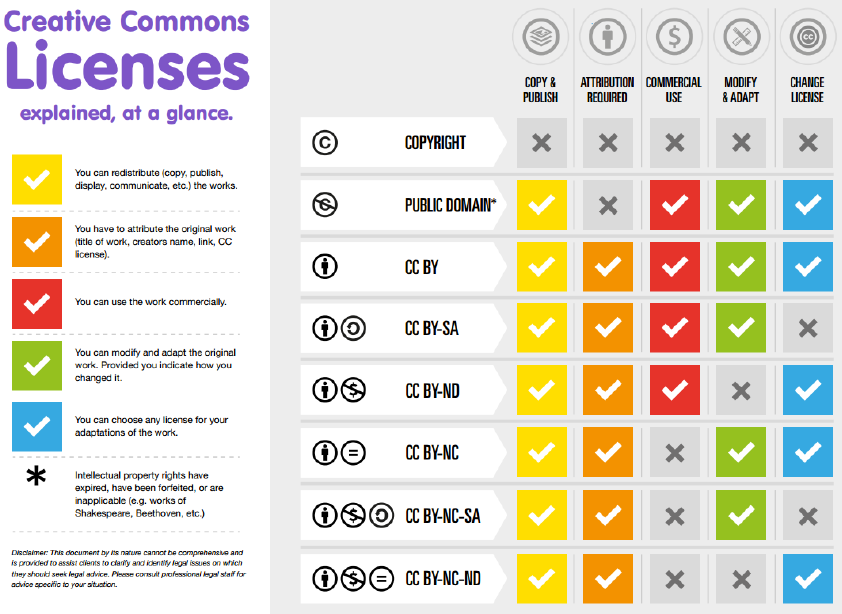
\includegraphics[width=150px]{img/OpenSource.png}
        \captionof{figure}{Abbildung Lizenzierungen}
        \label{fig:Abbildung Lizenzierungen}
\end{Figure}

\section{Urheberrechte (URG)}
\begin{itemize}
   \item \textbf{Werkbegriff (Art. 2 URG)}: Werke sind, unabhängig von ihrem Wert oder Zweck, \textbf{geistige Schöpfungen} der Literatur und Kunst, die \textbf{individuellen Charakter} haben
   \item Geschützt sind literarische, wissenschaftliche und andere Sprachwerke, Werke der Musik und andere akustische Werke sowie fotografische, kinematographische und andere visuelle oder audiovisuelle Werke, Werke der bildenden Kunst und der Baukunst sowie Computerprogramme
   \item Seit 1.4.2020: auch fotografische Wiedergaben und mit einem der Fotografie ähnlichen Verfahren hergestellte Wiedergaben dreidimensionaler Objekte gelten als Werke, auch wenn sie keinen individuellen Charakter haben (Art. 3 URG)
   \item Urheber (Art. 6 URG) können \textbf{nur natürliche} (nie juristische!) Personen sein. Mehreren Urhebern steht das Urheberrecht jedoch \textbf{gemeinschaftlich} zu
   \item Das Werk ist urheberrechtlich geschützt, \textbf{sobald es erschaffen ist}, unabhängig davon, ob es auf einem Träger festgehalten ist oder nicht (Art. 29 URG)
   \item Der Schutzt erlischt
   \subitem a.) \textbf{50 Jahre} nach dem Tod des Urhebers für Computerprogramme
   \subitem b.) \textbf{70 Jahre} nach dem Tod des Urhebers resp. letzten Urhebers 
\end{itemize}

\subsection{Inhalt des Urheberrechtes}
Grundsätzlich unterscheidet man zwischen
\begin{itemize}
   \item Urheber-\textbf{NUTZUNGS}-/Vewertungsrechte-Urheberrechte
   \item Urheber-\textbf{PERSÖNLICHKEITS}-Urheberrechte
   \item Urheber-\textbf{SONSTIGE-}Urheberrechte
\end{itemize}
\subsubsection{Verwertungsrechte}
Ausschliessliches Recht zu bestimmen, ob, wann und wie das Werk verwendet / verwertet wird (Art. 10 URG)

\subsubsection{Urheberpersönlichkeitsrechte}
Recht auf Anerkennung der Urhebergschaft und Bestimmung der Urheberbezeichnung, Erstveröffentlichtungsrecht, Recht auf Werkintegrität, Schutz vor Zerstörung (u.a. Art. 11 URG)

\subsubsection{Sonstige Rechte}
Zutritts- und Ausstellungsrecht (Art. 14 URG), Ausleih- und Vermietungstantiemen (Art. 13 Abs. 1 URG), Kopierabgabe (Art. 20 Abs. 2 URG)


\subsection{Urheberrechte des Arbeitnehmers}
\begin{itemize}
   \item Recht am Werk gehört grundsätzlich der (natürlichen) Person, die es erschaffen hat. Bei mehreren Personen steht es ihnen gemeinschaftlich zugreifen
   \item In der Regel (\textbf{muss!}) die Übertragung der Verwertungsrechte an den Arbeitgeber vertraglich geregelt werden. in Zweifelsfällen: \textit{Zweckübertragungstheorie} (Art. 16 Abs. 2 URG)
   \item ABER: wird in einem Arbeitsverhältnis bei Ausübung dienstlicher Tätigkeiten sowie in Erfüllung vertraglicher Pflichten ein Computerprogramm erschaffen, so ist der Arbeitgeber allein zur Ausübung der ausschliesslichen Verwendungsbefugnisse berechtigt (Art. 17 URG)
\end{itemize}
$\rightarrow$ Es spielt keine Rolle \textbf{wo, mit welchen Mittel, wann} die Software entwickelt wird. Wenn es in Ausübung seiner Arbeitstätigkeit (sehr schwammig) erfolgt, dann gehört es dem Arbeitsgeber.
Wenn man etwas entwickelt wofür man nicht angestellt ist, dann gehört es der Privatperson.

\subsection{Übertragung von Urheberrechten}
\begin{itemize}
   \item Die Übertragung des Urheberrechts erfolgt stets durch einen (Lizenz-)Vertrag (schriftlich oder mündlich oder stillschweigend)
   \item Liegt kein klarer Vertrag vor, so ist davon auszugehen, dass der Urheber seine Rechte nicht pauschal abtritt, sondern die Nutzung nur nach dem Zweckder Übertragung erlaubt (Zwecksübertragungstheorie)
\end{itemize}

\subsubsection{Beispiele}
Fotograf erstellt Fotos vom Firmenanlass für die interne Nutzung. Da die Fotos so toll geworden sind, möchte die Firma diese auch extern nutzen. Ist das zulässig?\\
$\rightarrow$ NEIN. Es war etwas anderes vereinbart (Zwecksübertragungstheorie)\\

Office365 für einen User und der User wird allen weitergegeben. Ist das zulässig?\\
$\rightarrow$ NEIN. Es war etwas anderes vereinbart (PER USER)

\subsection{Sonderregel für Software}
\begin{itemize}
   \item Art.10 Abs. 3 URG: Ausschliessliches Recht zur Vermietung
   \item Art 12 Abs. 2 URG: Erschöpfung, nur Weiterveräusserung oder Gebrauch
   \item Art.17 URG: Der Arbeitgeber hat ein Recht an den Programmen
   \item Art.19 Abs. 4 URG: Kein Eigengebrauch
   \item Art.21 URG: Entschlüsselung von Computerprogrammen
   \subitem 'legales hacking' jedoch nur unter bestimmten Voraussetzungen 
   \item Art.24 URG: Sicherungskopie
   \item Art.29 URG: Schutzdauer von 50 Jahren
\end{itemize}

\subsection{Rechtsschutz bei URG-Verletzung}
Man hat zwei Möglichkeiten (sowohl, als auch):
\begin{itemize}
   \item \textbf{Zivilrechtliche Ansprüche} Art. 61 ff. URG $\rightarrow$ allfälliges Geld fliesst zur Privatperson, jedoch Vorschuss notwendig
   \subitem Festellungsklage
   \subitem Unterlassungsklage
   \subitem Beseitigungsklage
   \subitem Klage auf Herkunftsangabe
   \subitem Schadenersatz
   \subitem Genugtuung
   \subitem Gewinnherausgabe
   \subitem Vorsorgliche Massnahmen 
   \item \textbf{Strafrechtliche Ansprüche} Art. 67 ff. URG $\rightarrow$ Durch Staatsanwalt (kostenlos im Interesse des Staates $\rightarrow$ allfälliges Geld fliesst in Staatskasse)
   \subitem Bei Vorsatz auf Antrag Gefängnis und Busse bis CHF 100'000.--
   \subitem Bei gewerbsmässiger Tatbegehung wird von Amtes wegen verfolgt 
\end{itemize}


\subsection{Gewährleistung 'Garantie'}
Man unterscheidet zwischen zwei unterschiedlichen Gewährleistungen

\subsubsection{Sachgewährleistung}
Der Lizenzgeber gewährleistet die Funktionalität des Lizenzgegenstandes mit den nachfolgenden Drittsoftware und das Testen sowie Anpassen des Lizenzgegenstandes bei Änderungen im Rahmen seiner üblichen Wartung

\subsubsection{Rechtsgewährleistung}
Behaupten Dritte Ansprüche, die den Auftraggeber hindern, die ihm vertraglich eingeräumten Nutzungsbefugnisse wahrzunehmen, unterrichtet der Auftraggeber den Auftragnehmer unverzüglich schriftlich und umfassen. Er ermächtigt den Auftragenehmer hiermit, Klagen gegen Dritte
gerichtlich und aussergerichtlich allein zu führen. Wird der Auftraggeber verklagt, stimmt er sich mit dem Auftragnehmer ab und nimmt Prozesshandlungen, insbesondere Anerkenntnisse und Vergleiche, nur mit dessen Zustimmung vor.
$\rightarrow$ Kommt heute sehr häufig vor



\chapter{Datenschutz}

\section{Weshalb Privacy und Datenschutz}
\begin{itemize}
   \item Menschen sind soziale Wesen - aber auch individualisten. Ständiger Konflikt zwischen beiden Naturen
   \item Wenn sie der liberalen Idee folgen, dass Menschen unabhängig sind - wer entscheidet, welche Infomrationen über eine Person wie benutzt werden dürfen?
   \item Menschliches Lernen beinhaltet Fehler zu machen. Was passiert, wenn die Gesellschaft sie ihr ganzes Leben immer wieder an lang zurückligendes Fehlverhalten erinnert?
   \item Privatsphäre ist ein Menschenrecht. ALle modernen Demokratien schützen diese
   \item Datenschutz bedeutet nicht Schutz von Daten
   \item Für die meisten Unternehmen gilt: grosse Reputationsrisiken, wenn Personendaten missbraucht werden.
\end{itemize}

\section{Wie könnte die Zukunft des Datenschutzes aussehen}
\begin{itemize}
   \item Zukunft: Totaler Kontrollverlust oder immer restriktiver
   \item AUf dem Papier haben die Menschen viele Rechte, aber auch in der Praxis?
   \item Daten sind (rechtlich) kein Eigentum - sie erzeugen nur einen Mehrwert, wenn sie genutzt werden
   \item Schutz würde auch bieten, wenn die Datensammler gesetzlich verpflichtet würden, andern (anonymisierte) Personendaten nutzen zu lassen. Analoges Beispiel :Open Banking Standard
   \item EU-Projekt: GAIA-X mit dem Ziel, eine sichere vertrauenswürdige Dateninfrastruktur aufzubauen
\end{itemize}

\section{Privacy - Spährentheorie}

\begin{itemize}
   \item Intimssphäre - Informationen, welche wir nicht nach aussen tragen wollen und uns evtl. schaden kann
   \item Friends-Zone - Schmerzt, wenn Informationen diese Zone verlassen, welche nicht raus sollten
   \item Halböffentlich - Keinen Schmerz, wenn die Information die Zone verlässt. Manchmal sogar erwünscht
\end{itemize}

\begin{Figure}
   \centering
    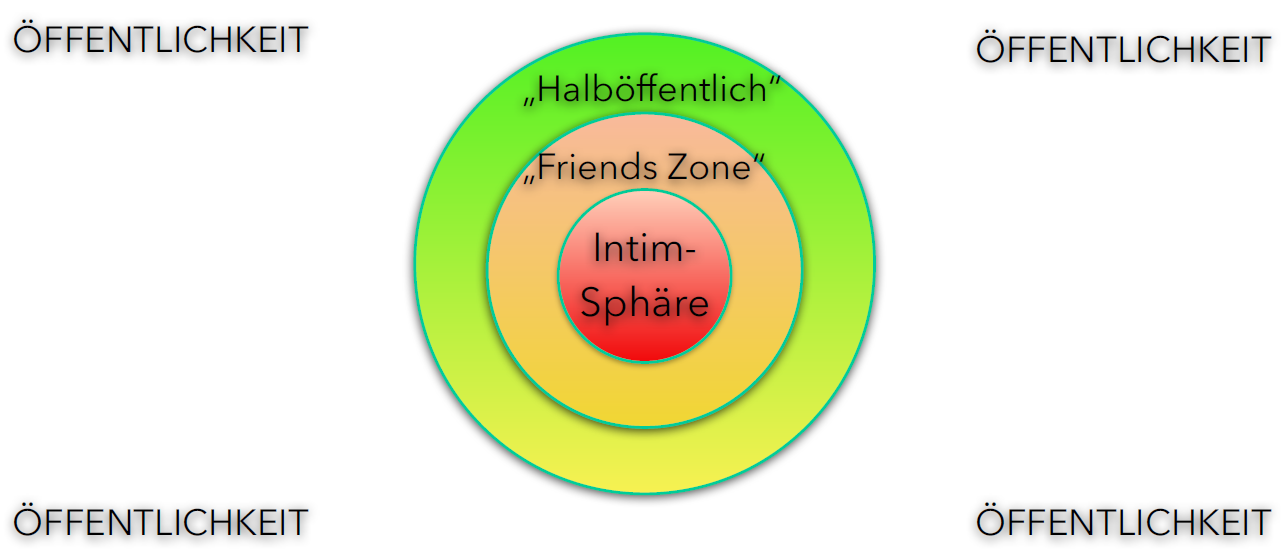
\includegraphics[width=150px]{img/Sphaerentheorie.png}
        \captionof{figure}{Abbildung der Sphaerentheorie}
        \label{fig:Abbildung der Sphaerentheorie}
\end{Figure}

\subsection{Integritätsschutz - Schutz der Persönlichkeit}
Jede Bearbeitung von Personendaten ist widerrechtlich. \\

Dabei gibt es drei Rechtfertigungsgründe, welches dies erlaubt:
\begin{enumerate}
   \item Einwilliung der Person / verletzten Personen
   \item Überwiegendes privates oder öffentliches Interesse
   \item Gesetzt welches dies erlaubt
\end{enumerate}

\textit{Beispiel:} Es ist ein überwiegendes privates Interesse zu wissen mit wem Sie die letzten 2 Wochen zusammen waren wegen dem COVID Tracing (nicht nur Geschäft?) $\rightarrow$ nicht zulässig

\section{Gesetzliches}

\subsection{Gesetzliche Grundlagen}
\begin{itemize}
   \item Schweizerische Bundesverfassung (Art. 13 BV)
   \item Schützt explizit die persönlichen Daten (Art. 27 / 28 ZGB) 
   \item Bundesgesetzt über den Datenschutz (DSG) und Verordnung dazu (VSDG)
   \item Zahlrecihe datenschutzrechtliche Bestimmungen in anderen Gesetzen (z.B. OR)
   \item Kantonales und Gemeinderecht: zahlreiche Gesetze und Verordnungen
   \item International: Europäische Datenschutzrichtlinie bzw. Grundverordnung
\end{itemize}

\subsection{Geltungsbereich - Art. 2 DSG}
\begin{enumerate}
   \item Dieses Gesetzt gilt für das Bearbeiten von Daten natürlicher und juristischer Personen durch
   \subitem private Personen (nDSG: nur noch natürliche Personen, kene juristische mehr)
   \subitem Bundesorgane
   \item Es ist nicht anwendbar auf
   \subitem Personendaten, die eine natürliche Person ausschliesslich zum pers. Gebraucht bearbeitet und nicht an Aussenstehende bekannt gibt
   \subitem Beratungen in den Eidgenössischen Räten und in den parlamentarischen Kommisssionen
   \subitem hängige Zivilprozesse, Strafverfahren, Verfahren der int. Rechtshilfe sowie staats- und verwaltungsrechtliche Verfahren mit Ausnahme erstinstanzlicher Verwaltungsverfahren
   \subitem öffentliche Register des Privatrechtsverkehrs
   \subitem Personendaten, die das int. Komitee vom Roten Kreuz bearbeitet
\end{enumerate}

\subsection{Begriffe und Defintiion}
tbd Slide 12 / 13 Datenschutz

\subsection{Datenschutzgrundsätze - Art 4 DSG}
\begin{enumerate}
   \item Personendaten dürfen nur rechtmässig bearbeitet werden
   \item Ihre Bearbeitung hat nach Treu und Glauben zu erfolgen und muss verhältnismässig sein
   \subitem verhältnismässig bedeutet die Waage zwischen dem Holen der privaten Daten under beabsichtigen Zweck. Die Frage ist dabei immer ob es einen solchen privaten Eingriffbraucht, um den Zweck zu erreichen 
   \item Personendaten dürfen nur zu dem Zweck bearbeitet werden, der bei der Beschaffung angegeben wurde, aus den Umständen ersichtlich oder gesetzlich vorgesehen ist
   \subitem Bspw. Contact-Tracing Zettel im Restaurant darf nur für das COVID Tracing verwendet werden, und nicht um bspw. Adressen zu speichern 
   \item Die Beschaffung von Personendaten und insbesondere der Zweck ihrer Bearbeitung müssen für die betroffene Person erkennbar sein
   \item Ist für die Bearbeitung von Personendaten die Einwilligung der betroffenen Person erforderlich, so ist diese Einwilligung erst gültig, wenn sie nach angemessener Information freiwillig erfolgt. Bei der Bearbeitung von besonders schützenswerten Personendaten oder Persönlichkeitsprofilen muss die Einwilligung zudem ausdrücklich erfolgen.
\end{enumerate}

\subsection{Richtigkeit der Daten - Art. 5 DSG}
\begin{enumerate}
   \item Wer Personendaten bearbeitet, hat sich über deren Richtigkeit zu vergewissern. Er hat alle angemessenen Massnahmen zu treffen, damit die Daten berichtigt oder vernichtet werden, die im Hinblick auf den Zweck ihrer Beschaffung oder Bearbeitung unrichtig oder unvollständig sind
   \item Jede betroffene Person kann verlangen, dass unrichtige Daten berichtigt werden
\end{enumerate}

\subsection{Grenzüberschreitende Bekanntgabe - Art. 6 DSG}
\begin{enumerate}
   \item Personendaten dürfen nicht ins Ausland bekannt gegeben werden, wenn dadurch die Persönlichkeit der betroffenen Personen schwerwigend gefährdet würde, namentlich weil eine Gesetzgebung fehlt, die einen angemessenen Schutz gewährleistet
   \item ... zahlreiche Voraussetzungen be ifehlen einer schützenden Gesetzgebung
\end{enumerate}
\textit{Beispiel:} CH Unternehmen mit Tochterunternehmen in der Trkei. Daten über Mitarbeiter werden hin und her gesendet, welche teilweise politische Meinung beinhaltet. Kann das problematisch sein?\\
$\rightarrow$ Ja, dies kann gerade in der Türkei gefährlich sein

\subsection{Datensicherheit - ART. 7 DSG}
\begin{enumerate}
   \item Personendaten müssen durch angemessene technische und organisatorische Massnahmen gegen unbefugtest Bearbeiten geschützt werden
   \item Der Bundesrat erlässt nähere Bestimmungen über die Mindestanforderungen an die Datensicherheit
\end{enumerate}

\subsection{Auskunftrecht - Art. 8 DSG}
\begin{enumerate}
   \item Jede Person kann vom Inhaber einer Datensammlung Auskunft darüber verlangen, ob Daten über sie bearbteitet werden
   \item Der Inhaber der Datensammlung muss der betroffenen Person mitteilen
   \subitem a) alle über sie in der Datensammlung vorhandenen Daten einschliesslich der verfügbaren Angaben über die Herkunft der Daten
   \subitem b) der Zweck und gegebenenfalls die Rechtsgrundlagen des Bearbeitens sowie die Kategorien der bearbeiteten Personendaten, der an der Sammlung Beteiligten under Datenempfänger
   \item Daten über die Gesundheit kann der Inhaber der Datensammlung der betroffenen Person durch einen von ihr bezeichneten Arzt mitteilen lassen
   \item Lässt der Inhaber der Datensammlung Personendaten durch einen Dritten bearbeiten, so bleibt er auskunftspflichtig. Der Dritte ist auskunftspflichtig, wenn er den Inhaber nicht bekannt gibt oder dieser keinen Wohnsitz in der Schweiz hat
   \item Die Auskunft ist in der Regel schriftlich, in Form eines Ausdrucks oder einer Fotokopie sowie kostenlos zu erteilen. Der Bundesrat regelt die Ausnahmen
   \item Niemand kann im Voraus auf das Auskunftsrecht verzichten
\end{enumerate}

\subsection{Einschränkung des Auskunftsrechtes - Art. 9 DSG}
\begin{enumerate}
   \item Der Inhaber der Datensammlung kann die Auskunft verweigern, einschränken oder aufschieben, soweit:
   \subitem a) ein Gesetz im formellen Sinn dies vorsieht;
   \subitem b) es wegen überwiegender Interessen Dritter erforderlich ist
   \item Ein Bundesorgan kann zudem die Auskunft verweigern, einschränken oder aufschieben soweit:
   \subitem a) es wegen überwiegender öffentlicher Interessen, insbesondere der inneren oder äusseren Sicherheit der Eidgenossenschaft erforderlich ist
   \subitem b) die Auskunft den Zweck einer Strafuntersuchung oder eines anderen Untersuchungsverfahrens in Frage stellt.
   \item Sobald der Grund für die Verweigerung, Einschränkung oder Aufschiebung einer Auskunft wegfällt, muss das Bundesorgan die Auskunft erteilen, ausser dies ist unmöglich oder nur mit einem unverhältnismässigem Aufwand möglich
   \item Der private Inhaber einer Datensammlung kann zudem die Auskunft verweigern, einschränken oder aufschieben, soweit eigene überwiegende Interessen es erfordern und er die Personendaten nicht Dritten bekannt gibt
   \item Der Inhaber der Datensammlung muss angeben, aus welchem Grund er die Auskunft verweigert, einschränkt oder aufschiebt. 
\end{enumerate}

\subsection{Datenbearbeitung durch Dritte - Art. 10A DSG}
\begin{enumerate}
   \item Das Bearbeiten von Personendaten kann durch Vereinbarung oder Gesetzt Dritten übertragen werden, wenn:
   \subitem a) die Daten nur so bearbeitet werden, wie der Auftraggeber selbst es tun dürfte; und
   \subitem b) keine gesetzliche oder vertragliche Geheimhaltungspflicht es verbietet
   \item Der Auftraggeber muss sich insbesondere vergewissern, dass der Dritte die Datensicherheit gewährleistet
   \item Dritte können dieselben Rechtfertigungsgründe geltend machen wie der der Auftraggeber 
\end{enumerate}

\subsection{Informationspflicht beim Beschaffen von besonders schützenswerten Personendaten und Persönlichkeitsprofilen - ART. 14 DSG}
\begin{enumerate}
   \item Der Inhaber der Datensammlung ist verpflichtet, die betroffene Person über die Beschaffung von besonders schützenswerten Personendaten oder Persönlichkeitsprofilen zu informieren; Diese Informationspflicht gilt auch dann, wenn die Daten bei Dritten beschafft werden.
   \item Der betroffenen Person sind mind. mitzuteilen:
   \subitem a) der Inhaber der Datensammlung
   \subitem b) der Zweck des Bearbeitens
   \subitem c) die Kategorien der Datenempfänger, wenn eine Datenbekanntgabe vorgesehen ist
   \item Werden die Daten nicht bei der betroffenen Person beschafft, so hat deren Information spätestens bei der Speicherung der Daten oder wenn die Daten nicht gespeichert werden, mit ihrer ersten Bekanntgabe an Dritte zu erfolgen
   \item Die Informationspflicht des Inhabers der Datensammlung entfällt, wenn die betroffene Person bereits informiert wurde oder, in Fällen nach Absatz 3, wenn
   \subitem a) die Speicherung oder die Bekanntgabe der Daten ausdrücklich im Gesetz vorgesehen ist; oder
   \subitem b) die Information nicht oder nur mit unverhältnismässigem AUfwand möglich ist.
   \item Der Inhaber der Datensammlung kann die Information unter den in Artikel 9 Absätze 1 und 4 genannten Voraussetzungen verweigern, einschränken oder aufschieben.  
\end{enumerate}

\subsection{Verletzung der Auskunfts-, Melde- und Mitwirkungspflichten - Art. 34 DSG}
\begin{enumerate}
   \item Mit Busse werden private Personen auf Antrag bestraft
   \subitem a) die ihre Pflichten nach den Artikeln 8-10 und 14 verletzten, indem sie vorsätzlich eine falsche oder eine unvollständige Auskunft erteilen
   \subitem b) die es vorsätzlich unterlassen:
   \subsubitem 1.) die betroffene Person nach Artikel 14 Absatz 1 zu informieren, oder
   \subsubitem 2.) ihr die Angaben nach Artikel 14 Absatz 2 zu liefern
   \item Mit Busse werden private Personen bestraft, die vorsätzlich:
   \subitem a) die Information nach Artikel 6 Absatz 3 oder die Meldung nach Artikel 11a unterlassen oder dabei vorsätzlich falsche Angaben machen;
   \subitem b) dem Beauftragten bei der Abklärung eines Sachverhaltes (Art. 29) falsche Auskünfte erteilen oder Mitwirkung verweigern
\end{enumerate}

\subsection{Arbeitsverhältnis und Datenschutz - Art. 328B OR}
Der Arbeitgeber darf Daten über den Arbeitnehmer nur
bearbeiten, soweit sie dessen Eignung für das
Arbeitsverhältnis betreffen oder zur Durchführung des
Arbeitsvertrages erforderlich sind. Im Übrigen gelten die
Bestimmungen des Bundesgesetzes vom 19. Juni 1992 über
den Datenschutz


\section{DSGVO aus Schweizer Sicht}
Die DSGVO ist seit Ende Mai 2018 auch für SChweizer Unternehmen direkt anwendbar, wenn:
\begin{itemize}
   \item Diese Waren oder DL in der EU/EWR anbieten (die Angabe des Preises in Euro genügt) und dazu personenbezognene Daten (bspw. Adressdaten, Kundenprofil) bearbeiten (Marktortprinzip: Art 3 Abs 2 DSGVO) oder
   \item diese das Verhalten von Website-Besuchern aus der EU sammeln und auswerten (Tracking durch Cookies, Profiling mit Tools wie Google Analytics, Facebook Pixel, etc.) oder
   \item diese regelmässige Newsletter an Empfänger in der EU versendet, oder
   \item diese im Auftrag oder als Konzernzentrale resp. -Mitglied eines in der EU domizilierten Unternehmens personenbezogene Daten bearbeiten
\end{itemize}
$\Rightarrow$ Wenn einer dieser Fälle auf ein Unternehmen zutrifft, besteht unmittelbar Handlungsbedarf

\begin{itemize}
   \item Grundsätzlich handelt es sich bei der DSGVO 'nur' um ein europäisch vereinheitliches Datenschutzrecht zur Durchetzung von mehrheitlich (auch bei uns) bereits bestehenden Grundsätzen
   \item Zur Durchsetzung können die EU-Aufsichtsbehörden nun aber Auskünfte und Überprüfungen veranlassen, Anweisungen erteilen sowie - bei wiederholter schwerer Missachtung - Geldbussen bis zu € 10 resp. 20 Mio. oder bis zu 2 resp 4 Prozent des weltweiten erzielten Jahresumsatzes verfügen. Die Massnahmen müssen jeweils aber verhältnismässig und wirksam sein. Bestragung von UNternehmen in der Schweiz sind noch unklar
   \item DSGVO ist nur ein 'Mindeststandard' EU-Länder können weitergehende Reglungen erlassen
\end{itemize}

Vereinfacht geht es um die Durchsetzung der (selbstverständlichen) Rechte der Bürger bezüglich:
\begin{itemize}
   \item Auskunftsrecht und Recht auf Datenübertragbarkeit
   \item Erweiterte Informationspflichten gegenüber der betroffenen Person
   \item Widerspruchsrecht
   \item Recht auf Löschung (Recht auf Vergessen)
   \item Möglihckeit für Abmahnungen und Klagen von Genugtuung und Schadenersatz für die betroffene Person
   \item Privacyby design und Privacy by default
   \item Erweiterte Dokumentationspflicht (TOM's, Verarbeitungsverzeichnisse)
\end{itemize}


\chapter{Domain-, Marken- und UWG-Recht}

\section{Markenrechte}
\begin{itemize}
   \item Markenrechte geben dem Inhaber \textbf{exklusive} Möglichkeit, sein Produkt oder seine Dienstleistung individuell zu kennzeichnen und jede Verwendung des Kennzeichens durch Dritte zu verhindern.
   \item Der nationale (!) Schutz entsteht durch Anmeldung und Eintragung des Kennzeichens für eine bestimmte Schutzklasse (d.h. Produkt- oder DL-Gruppe) im schweizerischen Markenregistert
   \item Der Markenschutz läuft nach 10 Jahren ab und kann beliebig oft erneuert werden. Voraussetzung ist, dass die Marke gewerblich benutzt wurde, ABER: die eingetragene Marke muss spätestens nach 5 Jahren markenmässig gebraucht werden, sonst verfällt der Schutz.
   \item Eine Marke ist ein Zeichen, das geeignet ist, Waren oder Dienstleistungen eines Unternehmens von andern Unternehmen zu unterscheiden. Marken können insbesondere Wörter, Buchstaben, Zahlen, bildliche Darstellungen, dreidimensionale Formen oder Verbindungen solcher Elemente untereinander oder mit Farbe sein (Art. 1 MSchG)
   \item Man unterscheidet zwischen:
   \subitem Wortmarken
   \subitem Bildmarken
   \subitem kombinierte Wort-/Bildmarken
   \subitem dreidimensionale Marken
   \subitem Hologramme
   \subitem Akustische Marken
   \subitem Farbmarken
   \subitem Positionsmarken
   \subitem Kollektivmarken (bspw. Raiffeisenbank)
   \subitem Garantiemarken (bspw. IP-Suisse)
\end{itemize}

\subsection{Absoluter Ausschluss des Markenschutzes}
\begin{itemize}
   \item Zeichen, die Gemeingut sind, es sei denn, dass sie sich als Marke für die Waren oder Dienstleistungen durchgesetzt haben, für die sie beansprucht werden
   \item Formen, die das Wesen der Ware ausmachen und Formen der Ware oder Verpackung, die technisch notwendig sind
   \item Irreführende Zeichen
   \item Zeichen, die gege die öffentliche Ordnung, die guten Sitten oder geltendes Recht verstossen (Art. 2 MSchG)
\end{itemize}

\subsection{relativer Ausschluss des Markenschutzes}
\begin{itemize}
   \item Zeichen, die mit einer älteren Marke identisch und für die gleichen Waren oder DL bestimmt sind wie diese
   \item Marken, die mit einer älteren identisch oder ähnlich sind und für gleichartige Waren oder DL bestimmt sind, so dass sich daraus eine Verwechslungsgefahr ergibt (Art. 3 MSchG)
\end{itemize}

\section{Gestzt über den unlauteren Wettbewerb (UWG)}
\textbf{Zweck:} Gewährleistung des lauteren ('fairen') und unverfälschten Wettbewerbs im Interesse aller am Markt Beteiligten\\
\textbf{Generaltatbestand} (Art. 2 UWG): \textit{Unlauter und widerrechtlich ist jedes täuschende oder in anderen Weise gegen den Grundsatz von Treu und Glauben verstossende Verhalten oder Geschäftsgebaren, welches das Verhältnis zwischen Mitbewerbern oder zwischen Anbietern und Abnehmer beeinflusst}\\

\subsection{Spezialtatbestande Art. 3-8 UWG}
\begin{itemize}
   \item \textbf{Herabsetzung und Anlehnung} an den Mitbewerber (Herabsetzung, Vergleich, Nachahmung, Anlehnung)
   \item \textbf{Irreführung}
   \item \textbf{Einwirken} auf den \textbf{Willen} eines Dritten zwecks Abschluss eines Vertrages
   \item \textbf{Verleihung} zu \textbf{Vertragsbruch}
   \item \textbf{Verwertung fremder Arbeitsergebnisse}
   \item \textbf{Verletzung} von \textbf{Fabrikations-} und \textbf{Geschäftsgeheimnisse}
   \item \textbf{Verwendung missbräuchlicher Geschäftsbedingungen} (AGB)
   \item \textbf{Spam-Verbot} (Art. 3 Abs. 1 lit. o UWG)
   \item Formvorschriften für (entgeltliche) Eintragung in Verzeichnisse (Art. 3 Abs. 1 lit. p UWG)
   \item \textbf{Verbot von Schneeball-, Lawinen- oder Pyramidensystemen} (Art. 3 Abs. 1 lit. r UWG)
   \item \textbf{Impressungspflicht im elektronischen Geschäftsverkehr} (Art. 3 Abs. 1 lit. s UWG)
   \item Verbot für überteuerte Mehrwertdienstnummern bei Wettbewerben (Art. 3 Abs. 1 lit. t UWG)
   \item Verbot von Adressweitergabe (Art. 3. Abs. 1 lit. u UWG)
\end{itemize}

\subsection{Rechtsschutz bei UWG-Verletzungen}
\textit{zivilrechtliche Ansprüche} (Art. 9 ff UWG):
\begin{itemize}
   \item Feststellungsklage
   \item Unterlassungsklage
   \item Beseitigungsklage
   \item Klage auf Herkunftsangabe
   \item Schadenersatz
   \item Genugtuung
   \item Gewinnherausgabe
   \item Vorsorgliche Massnahmen
\end{itemize}

\textit{Strafrechtliche Ansprüche} (Art. 23 ff UWG): Bei Vorsatz auf Antrag \textbf{Gefängnis und Busse bis CHF 100'000}. Bei gewerbsmässiger Tatbegehung wird von Amtes wegen verfolgt

\chapter{Strafrecht}

Weshalb braucht es Strafrecht?
\begin{itemize}
   \item Gewaltmonopol des Staates als stabilisierende, kulturelle Leistung. Aber nur, wenn Monopol demokratisch legitimiert ist und Verfahren und Sanktionen voraussehbar sind! Ziel des Strafrechtes ist u.a. Abschreckung (Generalprävention) und indvidiuelle Besserung (Spezialprävention)
   \subitem Demokratisch legitimiert
   \subitem Eng umschrieben, was der Staat tun darf und was nicht 
   \item nulla poene sine lege (keine Strafe ohne Gesetz)
   \subitem Wenn neue Delikte auftauschen und es noch kein Gesetz dafür gibt, kann das Gericht nicht einfach neue Strafen erfinden 
   \item Bestraft wird nur, wem tatbestandmässiges, rechtswidriges und schuldhaftes Handeln nachgewiesen wurde
\end{itemize}

\section{Verbrechensmerkmale}
\begin{enumerate}
   \item Menschliche Handlung
   \subitem bspw. wenn der Hund etwas macht, wird der Halter strafrechtlich belangt und nicht der Hund 
   \item Tatbestandmässig (objektiv / subjektiv)
   \subitem objektiv $\rightarrow$ Was ist tatsächlich passiert?
   \subitem subjektiv $\rightarrow$ vorsätzlich / eventualvorsätzlich / fahrlässig (grob- oder leichtfahrlässig)
   \item Rechtswidrig (Notwehr / Notstand)
   \subitem Man muss etwas machen, um sein Leben zu retten (bspw. wird mit einer Pistole bedroht und man greift zu einem Gegenstand und tötet den Gegenüber) $\rightarrow$ hebt diese Rechtslage auf 
   \item Schuldhaft (Schuldfähigkeit)
   \subitem schuldunfähig / verminderte Schuldfähigkeit 
   \subitem bspw. beteiligt beim Tod einer Person, aber man hatte keinen Einfluss darauf nehmen können.
   \item Mit Strafe / Sanktion bedroht
\end{enumerate}

\subsection{Anstiftung und Mitwirkung}
\textbf{Anstiftung:} Jemand anderen zur Ausübung eines Verbrechens oder Vergehens motivieren.\\
\textbf{Mitwirkung:} wesentlichen Tatbeitrag mitliefern\\
$\rightarrow$ beides ist Strafbar. Grundsätzlich wird der Anstifer und Mittäer wie der Haupttäter bestraft. Also auch dann, wenn er ander Tat nicht unmittelbar beteiligt war.

\subsection{Sanktionen}
Strafen:
\begin{itemize}
   \item Freihheitsstrafen (Vergehen $\leq$ 3 Jahre / Verbrechen $\geq$ 3 Jahre)
   \subitem 3 Tage - 20 Jahren, z.T. lebenslänglich 
   \item Geldstrafe
   \subitem 1 - 360 Tagessätze 
   \item Gemeinnützige Arbeit
   \subitem 0 - 729 Stunden
   \item Busse
   \subitem 0 - 10'000.-- 
\end{itemize}
$\rightarrow$ eine bedingte Strafe kann mit einer unbedingten Geldstrafe / Busse verbunden werden\\

Massnahmen:
\begin{itemize}
   \item therapeutische Massnahme (stationär / ambulant)
   \item Verwahrung
   \item andere (Berufsverbot / Fahrverbot / Einziehung etc.)
\end{itemize}

\section{Ablauf Strafverfahren}
\begin{enumerate}
   \item Polizei / Staatsanwaltschaft wird aktiv
   \item Untersuchungsleitung durch Staatsanwaltschaft
   \item Staatsanwaltschaft hat Aufgabe, belastende und entlastende zu untersuchen (Im Zweifel klagt er jedoch an)
   \item Entscheidet, ob Fall zur Beurteilung an Strafgericht überwiesen wird
   \item Staatsanwaltschaft hat in einfachen Fällen Strafkompetenz (Busse, Geldstrafe bis 180 Taggelder, Haft bis max. 6 Monate)
\end{enumerate}

\chapter{Cyber-Kriminalität}

Typische Cyber-Delikte
\begin{itemize}
   \item Unbefugte Datenbeschaffung (143 StGB)
   \item Unbefugtes Eindringen (Hacken) in Datenverarbeitungssystem (143bis StGB)
   \item Datenbeschädigung (144 StGB)
   \item Betrügerischer Missbrauch einer Datenverarbeitungsanlage (147 StGB)
   \item Herstellen und Inverkehrberingen von Materialien zur unbefugten Entschlüsselung codierter Angebote (150Bis StGB)
   \item Verletzung des Fabrikations- oder Geschäftsgeheimnissess (162 StGB)
   \item Ehrverletzungen (173 ff StGB)
   \item Verletzung des Schriftgeheimnisses (179 StGB)
   \item Unbefugtes Beschaffen von Personendaten (179novies StGB)
   \item Pornografie (197 StGB)
   \item Störung von Betrieben, die der Allgemeinheit dienen (239 StGB)
   \item Rassendiskriminierung (261bis StGB)
   \item Wirtschaftlicher Nachrichtendienst (273 StGB)
\end{itemize}

KOBIK = nationale Koordinationsstelle zur Bekämpfung der Internetkriminalität

\section{Ausführungen einzelner Artikel}

\subsection{Unbefugte Datenbeschaffung - Art. 143 StGB}
\begin{enumerate}
   \item Wer in der Absicht, sich oder einen anderen unrechtmässig zu bereichern, sich oder einem anderen elektronisch oder in vergleichbarer Weise gespeicherte oder übermittelte Daten beschafft, die nicht für ihn bestimmt und  gegen sein unbefugten Zugriff besonders gesichert sind, wird mit Freihheitsstrafe bis zu fünf Jahren oder Geldstrafe bestraft Die unbefugte Datenbeschaffung zum Nachteil eines Angehörigen oder Familiengenossen wird nur auf Antrag verfolgt
\end{enumerate}

\subsection{Unbefugtes Eindringen in ein Datenverarbeitungssystem - Art. 143bis StGB}
\begin{enumerate}
   \item Wer auf dem Wege von Datenübertragungseinrichtungen unbefugterweise in ein fremdes, gegen seinen Zugriff besonders gesichertes Datenverarbeitungssystem eindringt, wird, auf Antrag, mit Freihheitsstrafe bis zu drei Jahren oder Geldstrafe bestraft
   \item Wer Passwörter, Programme oder andere Daten, vondenen er weiss oder annehmen muss, dass sie zur Begehung einer strafbaren Handlung gemäss Absatz 1 verwendet werden soll, in Verkehr bringt oder zugänglich macht, wird mit Freihheitsstrafe bis zu drei Jahren oder Geldstrafe bestraft
\end{enumerate}

\subsection{Datenbeschädigung - Art. 144bis StGB}
\begin{enumerate}
   \item Wer unbefugt elektronisch oder in vergleichbarer Weise gespeicherte oder übermittelte Daten verändert, löscht oder unbrauchbar macht, wird, auf Antrag, mit Freihheitsstrafe bis zu drei Jahren oder Geldstrafe bestraft
   \subitem Hat der Täter einen grossen Schaden verursacht, so kann auf Freihheitsstrafe von einem Jahr bis zu fünf Jahren erkannt werden. Die Tat wird von Amtes wegen verfolgt.
   \item Wer Programme von denen er weiss oder annehmen muss, dass sie zzu den in Ziffer 1 genannten Zwecken verwendet werden sollen, herstellt, einführt, in Verkehr bringt, anpreist, anbietet oder sonst wie zugänglich macht oder zu ihrer Herstellung Anleitung gibt, wird mit Freiheitsstrafe bis zu drei Jahren oder Geldstrafe bestraft
   \subitem Handelt der Täter gewerbsmässig, so kann auf Freihheitsstrafe von einem Jahr bis zu fünf Jahren erkannt werden.  
\end{enumerate}

\subsection{Betrügerischer Missbrauch einer Datenverarbeitungsanlage - Art. 147 StGB}
\begin{enumerate}
   \item Wer in der Absicht, sich oder einen anderen unrechtmässig zu bereichern, durch unrichtige, unvollständige oder unbefugte Verwendung von Daten oder in vergleichbarer Weise auf einen elektronischen oder vergleichbaren Datenverarbeitungs- oder Datenübermittlungsvorgang einwirkt und dadurch eine Vermögensverschiebung zum Schaden eines anderen herbeiführt oder eine Vermögensverschiebung unmittelbar danach verdeckt, wird mit Freihheitsstrafe bis zu fünf Jahren oder Geldstrafe bestraft
   \item Handelt der Täter gewerbsmässig, so wird er mit Freihheitsstrafe bis zu zehn Jahren oder Geldstrafte nicht unter 90 Tagessätze bestraft
   \item Der betrügerische Missbrauch einer Datenverarbeitungsanlage zum Nachteil eines Angehörigen oder Familiengenossen wird nur auf Antrag verfolgt
\end{enumerate}

\subsection{Herstellen ung Inverkehrbringen von Materialien zur unbefugten Entschlüsselung codierter Angebote - Art. 150bis StGB}
\begin{enumerate}
   \item Wer Geräte, deren Bestandteile oder Datenverarbeitungsprogramme, die zur unbefugten Entschlüsselung codierter Rundfunkprogramme oder Fernmeldedienste bestimmt und geeignet sind, herstellt, einführt, ausführt, durchführt, in Verkehr bringt oder installiert, wird, auf Antrag, mit Busse bestraft
   \item Versuch und Gehilfenschaft sind strafbar
\end{enumerate}

\subsection{Ehrverletzungs-Delikate - Art. 173 / 174 / 177 StGB}
\textbf{Üble Nachrede - Art. 173 StGB}:\\
Der Straftatbestand hat zum Ziel, jemanden zu bestrafen, der gegenüber einem Dritten über eine andere Person rufschädigende vorsätzlich wahre oder unvorsätzlich unwahre Äusserungen tätigt oder weiterverbreitet. Der Täter kann sich allerdings entlasten und bleibt straflos, wenn ihm der sogenannte Entlastungsbeweis gelingt\\

\textbf{Verleumdung - Art. 174 StGB}:\\
Die Verleumdung ist üble Nachrede wider besseres Wissens. Der Täter beschudligt oder verdächtigt einen Person gegenüber einen Dritten eines unehrenhaften Verhaltens oder anderer rufschädigender Tatsachen, die in Wirklichkeit nicht bestehen und somit unwahr sind. Der Entlastungsbeweis ist nicht möglich.\\

\textbf{Beschimpfung - Art. 177 StGB}:\\
Der Beschimpfung macht sich strafbar, wenn jemand in anderer Weise - d.h. nicht durch üble Nachrede oder Verleumdung - durch Wort, Schrift, Bild, Gebärde oder Tätlichkeiten in der Ehre angegriffen wird.

\subsubsection{Social Media}
Auch das Liken in Social Media kann gemäss dem Urteil des Bezirksgericht Zürich strafbar sein. Dieser Entscheid wurde ebenfalls durch die zweite, wie auch die Dritte Instanz bestätigt.

\section{Nationales Zentrum für Cybersicherheit - NCASC (Ehemalig MELANI)}
Das Nationale Zentrum für Cybersicherheit (NCSC) ist das Kompetenzzentrum des Bundes für Cybersicherheit und damit erste Anlaufstelle für die Wirtschaft, Verwaltung und Bildungseinrichtungen und die Bevölkerung bei Cyberfragen.\\
Als strafrechtlich relevant gelten Inhalte im Internet, die eines der nachstehenden Merkamle aufweisen (nicht abschliessend):
\begin{itemize}
   \item harte Pornografie (sexuelle Handlungen mit Kindern, Tieren, menschlichen Ausscheidungen oder Gewaltätigkeit)
   \item legale Pronografie, die auch von Minderjährigen konsumiert werden kann, wenn weder ein Kinderschutz noch eine Alterskontrolle angeboten wird
   \item Gewaltdarstellung
   \item Rassimus, Extremismus
   \item Ehrverletzungen, Drohungen
   \item Betrug, Wirtschaftsverbrechen
   \item unbefugtes Eindringen in Computersyteme, Verbreitung von Computerviren, Datenbeschädigung
\end{itemize}

\chapter{relevante Gesetzesartikel}

\section{Allgemeines und Verträge}
\begin{tabular}[h]{p{0.15\linewidth}|p{0.25\linewidth}|p{0.50\linewidth}}
   \textbf{Gesetzesartikel} & \textbf{Titel} & \textbf{Beschreibung} \\
   \hline
   BV Art. 1 & Bundesverfassungsgrundsatz & Das Schweizervolk und die Kantone, bilden die Schweizerische Eidgenossenschaft und nicht umgekehrt\\
   \hline
   BV Art. 13 & Schutz der Privatsphäre & tbd \\
   \hline
   ZGB Art. 1 & Rechtsquelle & geschriebenes Recht, Gewohnheitsrecht, Gerichtspraxis\\
   \hline
   ZGB Art. 2 & Vermutung des guten Glaubens & Handeln nach Treu und Glauben\\
   \hline
   ZGB Art. 4 & Richterliches Ermessen & Der Richter hat die Möglichkeit, sein eigenes Ermessen mit einzubringen\\
   \hline
   ZGB Art. 8 & Beweislast & Es muss eine Beweislast vorliegen\\
   \hline
   ZGB Art. 27 & Schutz der Persönlichkeit & tbd \\
   \hline
   ZGB Art. 28 & Integritätsschutz & Wer in seiner Persönlichkeit widerrechtlich verletzt wird, kann zu seinem Schutz gegen jeden, der in der Verletzung mitwirkt, das Gericht anrufen \\
   \hline
   OR Art. 1 & Vertragsabschluss & Vertrag kommt durch gegenseitige, übereinstimmende Willensäusserung zustande. Diese kann ausdrücklich oder stillschweigend erfolgen.\\
   \hline
   OR Art. 7 & Antrag ohne Verbindlichkeit & Verbindliche Offerte oder bloss Einladung zur Offertstellung \\
   \hline
   OR Art. 11 & Formvorschrift & Verträge sind grundsätzlich an keine Form gebunden, ausser das Gesetz verlangt es $\Rightarrow$ Formlos, Einfache Schriftlichkeit, Qualifizierte Schriftlichkeit, Öffentliche Beurkundung, Eintrag in ein öffentliches Register, Öffentliche Beurkundung und Eintrag in öffentliches Register \\
   \hline
   OR Art. 91 & Verzug des Gläubigers & Der Gläubiger kommt in Verzug, wenn er die Annahme der gehörig angebotenen Leistung oder die Vornahme der ihm obliegenden Vorbereitungshandlungen, ohne die der Schuldner zu erfüllen nicht imstande ist, ungerechtfertigterweise verweigert. \\
   \hline
   OR Art. 102 & Verzug des Schuldners & Ist eine Verbindlichkeit fällig, so wird der Schuldner durch Mahnung des Gläubigers in Verzug gesetzt. Bei Verabredung zu Verfalltag, kommt der Schuldner mit Ablauf in den Verzug.\\
   \hline
   OR Art. 103ff. & Verzugsfolgen allgemein & Schadenersatz etc.\\
   \hline
   OR Art. 197 & Gewährleistung wegen Mangel der Kaufsache & Verkäufer haftet dem Käufer für die zugesicherten Ware (körperliche und rechtliche Mangel), auch wenn er Mangel nicht gekannt hat \\
   \hline
   OR Art. 328b & Arbeitsverhältnis und Datenschutz & Der Arbeitgeber darf Daten über den Arbeitnehmer nur bearbeiten, soweit sie dessen Eignung für das Arbeitsverhältnis betreffen oder zur Durchführung des Arbeitsvertrages erforderlich sind. \\
   \hline
   OR Art. 367 & Haftung für Mängel & tbd \\
   \hline
   OR Art. 404 & Auflösung Auftragsverhältnis & Kann jederzeit aufgelöst werden, jedoch nicht zu einer Unzeit \\
   \hline
\end{tabular}

\section{Urheberrecht}
\begin{tabular}[h]{p{0.15\linewidth}|p{0.25\linewidth}|p{0.50\linewidth}}
   \textbf{Gesetzesartikel} & \textbf{Titel} & \textbf{Beschreibung} \\
   \hline
   URG Art. 2 & Werkbegriff & Werke sind unabhängig von ihrem Werk oder Zweck, geistige Schöpfungen der Literatur und Kunst, die individuellen Charakter haben \\
   \hline
    URG Art. 3 & Fotografie als Werk & auch fotografische Wiedergaben und mit einem der Fotografie ähnlichen Verfahren hergestellte Wiedergaben dreidimensionaler Objekte gelten als Werke, auch wenn sie keinen individuellen Charakter haben \\
   \hline 
   URG Art. 6 & Urheber Personen & Können nur natürliche und nie juristische Personen sein. Bei mehreren Urheber steht das Urheberrecht jedoch gemeinschaftlich zu \\
   \hline
   URG Art. 10 & Verwertungsrechte-Urheberrechte & Ausschliessliches Recht zu bestimmen, ob, wann und wie das Werk verwendet / verwertet wird \\
   \hline
   URG Art. 10 Abs. 3 & Ausschliessliches Recht zur Vermietung & tbd \\
   \hline
   URG Art. 11 & Urheberpersönlichkeitsrechte & Recht auf Anerkennung der Urhebergschaft und Bestimmung der Urheberbezeichnung, Erstveröffentlichtungsrecht, Recht auf Werkintegrität, Schutz vor Zerstörung\\
   \hline
   URG Art. 12 Abs. 3 & Erschöpfng, nur Weiterveräusserung oder Gebrauch & tbd \\
   \hline
   URG Art. 13 Abs. 1 & Ausleih- und Vermietungstantiemen & tbd \\
   \hline
   URG Art. 14 & Zutritts- und Ausstellungsrecht & tbd\\
   \hline
   URG Art. 16 Abs. 2 & Zwecksübertragungstheorie & I.d.R. muss die Übertragung der Verwertungsrechte an den Arbeitgeber vertraglich geregelt werden. In Zweifelsfällen: Zwecksübertragungstheorie\\
   \hline
   URG Art. 17 & Arbeitgeber hat Recht an den Programmen &  Wird in einem Arbeitsverhältnis bei Ausübung dienstlicher Tätigkeiten sowie in Erfüllung vertraglicher Pflichten ein Computerprogramm erschaffen, so ist der Arbeitgeber allein zur Ausübung der ausschliesselichen Verwendungsbefugnisse berechtigt. \\
   \hline
   URG Art. 19 Abs. 4 & Kein Eigengebraucht & tbd \\
   \hline
   URG Art. 20 Abs. 2 & Kopierabgabe & tbd\\
   \hline
   URG Art. 21 & Entschlüsselung von Computerprogrammen & tbd \\
   \hline
   URG Art. 24 & Sicherungskopie & tbd \\
   \hline
   URG Art. 29 & Zeitpunkt des Schutzes & Das Werk ist urheberrechtlich geschtützt, sobald es erschaffen ist, unabhängig davon, ob es auf einem Träger festgehalten ist oder nicht \\
   \hline
   URG Art. 29 & Dauer des Schutzes & erlischt nach 50 Jahren nach dem Tod des Urhebers für Computerprogramme und nach 70 Jahre nach dem Tod des Urhebers resp. letzten Urhebers \\
   \hline
   URG Art. 61 ff. & Zivilrechtliche Ansprüche & Feststellungsklage, Unterlassungsklage, Beseitigungsklage, Klage auf Herkunftsangabe, Schadenersatz, Genugtuung, Gewinnherausgabe, Vorsorgliche Massnahme \\
   \hline
   URG Art. 67 & Strafrechtliche Ansprüche & Bei Vorsatz auf Antrag Gefängnis und Busse bis 100k; Bei gewerbsmässiger Tatbegehung wird von Amtes wegen verfolgt \\
\end{tabular}

\section{Datenschutzgesetz}
\begin{tabular}[h]{p{0.15\linewidth}|p{0.25\linewidth}|p{0.50\linewidth}}
   \textbf{Gesetzesartikel} & \textbf{Titel} & \textbf{Referenz in ZF} \\
   \hline
   DSG Art. 2 & Geltungsbereich & Kapitel 4.4.2 S. 16 \\
   \hline
   DSG Art. 4 & Datenschutzgrundsätze & Kapitel 4.4.4 S. 16 \\
   \hline
   DSG Art. 5 & Richtigkeit der Daten & Kapitel 4.4.5 S. 17 \\
   \hline
   DSG Art. 6 & Grenzüberschreitende Bekanntgabe & Kapitel 4.4.7 S. 17 \\
   \hline
   DSG Art. 7 & Datensicherheit & Kapitel 4.4.6 S. 17 \\
   \hline
   DSG Art. 8 & Auskunftsrecht & Kapitel 4.4.8 S. 17 \\
   \hline
   DSG Art. 9 & Verweigerung Auskunftsrecht & Kapitel 4.4.9 S. 17 \\
   \hline
   DSG Art. 10a & Datenbearbeitung durch Dritte & Kapitel 4.4.10 S. 17 \\
   \hline
   DSG Art. 14 & Informationspflicht beim Beschaffen & Kapitel 4.4.11 S. 18 \\
   \hline
   DSG Art. 34 & Verletzung der Auskunfts-, Melde- und Mitwirkungspflichten & Kapitel 4.4.10 S. 18 \\
   \hline
   DSGVO Art. 3 Abs. 2 & Marktortprinzip & Ware oder DL in EU anbietet (in Euro genügt) und dazu personenbezogene Daten bearbeitet - Kapitel 4.5\\
   \hline
   OR Art. 328b & Arbeitsverhältnis und Datenschutz & Kapitel 4.4.12 S. 18 \\
\end{tabular}

\section{Domain-, Marken- und UWG-Recht}
UWG = Unlauter Wettbewerb\\
\begin{tabular}[h]{p{0.15\linewidth}|p{0.25\linewidth}|p{0.50\linewidth}}
   \textbf{Gesetzesartikel} & \textbf{Titel} & \textbf{Beschreibung} \\
   \hline
   MSchG Art. 1 & Marke & Eine Marke ist ein Zeichen, das geeignet ist, Waren oder Dienstleistungen eines Unt. von anderen Unt. zu unterscheiden.\\
   \hline
   MSchG Art. 2 & absoluter Auschluss & Gemeingut, irreführende Zeichen oder Zeichen gegen die öffentliche Ordnung, die guten Sitten oder geltendes Recht verstossen.\\
   \hline
   MSchG Art. 3 & relativer Ausschluss & Marken, die mit einer älteren Marke identisch oder ähnlich sind für gleichartige Waren oder DL bestimmt sind, so dass sich daraus eine Verwechslungsgefahr ergibt.\\
   \hline
   UWG Art. 2 & Generaltatbestand & Unlauter und widerrechtlich ist jedes täuschende oder in anderen Weise gegen den Grundsatz von Treu und Glaube verstossende Verhalten oder Geschäftsgebaren, welches das Verhältnis zwischen Mitbewerbern oder zwischen Anbietern und Abnehmer beeinflusst.\\
   \hline
   UWG Art. 3 Abs. 1 lit. o & Spam-Verbot Spezialtatbestand & tbd\\
   \hline
   UWG Art. 3 Abs. 1 lit. p & Formvorschriften für Eintragung in Verzeichnisse Spezialtatbestand & tbd\\
   \hline
   UWG Art. 3 Abs. 1 lit. r & Schnellball/Pyramidensystemen-Verbot Spezialtatbestand & tbd\\
   \hline
   UWG Art. 3 Abs. 1 lit. s & Impressungspflicht bei elek. Geschäftsverkehr Spezialtatbestand & tbd\\
   \hline
   UWG Art. 3 Abs. 1 lit. u & Verbot der Adressweitergabe Spezialtatbestand & tbd\\
   \hline
   UWG Art. 3 Abs. 1 lit. o & Spam-Verbot Spezialtatbestand & tbd\\
   \hline
   UWG Art. 9ff. & Zivilrechtliche Ansprüche & Feststellungsklage, Unterlassungsklage etc. \\
   \hline
   UWG Art. 23ff.& Strafrechtliche Ansprüche & Bei Vorsatz auf Antrag Gefängnis und Busse bis CHF 100k. Bei gewerbsmässiger Tatbegehung wird von Amteswegen verfolgt\\
\end{tabular}

\section{Strafrecht / Cyber-Kriminalität}

\begin{tabular}[h]{p{0.15\linewidth}|p{0.25\linewidth}|p{0.50\linewidth}}
   \textbf{Gesetzesartikel} & \textbf{Titel} & \textbf{Beschreibung} \\
   \hline
   StGB Art. 143 & Unbefugte Datenbeschaffung & Wer in der Absicht, sich oder einen anderen unrechtmässig zu bereichen (...) elektronisch oder in vergl. Weise gespeicherte oder übermittelte Daten beschafft (...) $\rightarrow$ Referenz Kapitel 7.1.1 Seite 24\\
   \hline
   StGB Art. 143bis & Unbefugtes Eindringen in ein Datenverarbeitungssystem & (...)auf dem Wege (...) unbefugterweise in ein fremdes, gegen seinen Zugriff besonders gesichertes Datenverarbeitungssystem eindringt, wird, \textbf{auf Antrag} mit Freiheitsstrafe bis 3 Jahren oder Geldstrafe $\rightarrow$ Referenz Kapitel 7.1.2 Seite 25\\
   \hline
   StGB Art. 144bis & Datenbeschädigung & (...) gespeicherte oder übermittelte Daten verändert, löscht oder unbrauch macht, wird, auf \textbf{Antrag} mit bis zu 3 Jahren (schweren Fällen bis 5) oder Geldstrafe $\rightarrow$ Referenz Kapitel 7.1.3 Seite 25\\
   \hline
   StGB Art. 147bis & Betrügerischer Missbrauch & (...) unrechtmässig zu bereichern, durch unrichtige, unvollständige oder unbefugte Verwendung von Daten (...) bis zu 5 Jahren $\rightarrow$ Referenz Kapitel 7.1.4 Seite 25\\
   \hline
   StGB Art. 150 & Herstellen und Inverkehrbringen zur unbefugten Entschlüsselung codierter Angebote & (...) unbefugten Entschlüsselung codierter Rundfunkprogramme oder Fernmeldedienste bestimmt und geeignet sind, herstellt, einführt, ausführt, durchführt, in Verkehr bringt oder installiert, wird, \textbf{auf Antrag}, mit Busse bestraftn $\rightarrow$ Referenz Kapitel 7.1.5 Seite 25 \textbf{Wichtig:} Versuch und Gehilfeschaft ist strafbar\\
   \hline
   StGB Art. 173 & üble Nachrede & (...) gegenüber einem Dritten über eine andere Person rufschädigende vorsätzliche wahre oder unvorsätzlich unwahre Äusserungen tätig oder weiterverbreitet $\rightarrow$ Referenz Kapitel 7.1.6 Seite 25\\
   \hline
   StGB Art. 174 & Verleumdung & Die Verleumdung ist üble Nachrede wider besseres Wissens. (...) eines unehrenhaften Verhaltens oder rufschädigender Tatsachen, die in Wirklichkeit nicht bestehen und somit unwahr sind. Der Entlastungsbeweis ist nicht möglich. $\rightarrow$ Referenz Kapitel 7.1.6 Seite 25\\
   \hline
   StGB Art. 177 & Beschimpfung & Der Beschimpfung macht sich strafbar, wenn jemand in anderer Weise - d.h. nicht durch üble Nachrede oder Verleumdung - durch Wort, Schrift, Bild, Gebärde oder Tätlichkeiten in der Ehre angegriffen wird $\rightarrow$ Referenz Kapitel 7.1.6 Seite 26\\
\end{tabular}

\textbf{Abgrenzungen und Anwendungsfälle}
\begin{itemize}
   \item Auch das Liken in Social Media kann gemäss dem Urteil des Bezirksgericht Zürich strafbar sein. Dieser Entscheid wurde ebenfalls durch die zweite, wie auch die Dritte Instanz bestätigt.
   \item Üble Nachrede beim Journalismus? \textit{Natürlich wäre der Journalist gemäss Art. 173 StGB strafbar, wenn er wahre ehrverletzende Dinge über jemanden schreibt. ABER es gibt Art. 173 Ziffer 2: "Beweist der Beschuldigte, dass die von ihm vorgebrachte oder weiterverbreitete Äusserung der Wahrheit entspricht, oder dass er ernsthafte Gründe hatte, sie in guten Treuen für wahr zu halten, so ist er nicht strafbar." (sog. "Gutglaubensbeweis").}
\end{itemize}


\end{document}